%%% Version 3.4 Generated 2022/06/14 %%%
%%% You will need to have the following packages installed: datetime, fmtcount, etoolbox, fcprefix, which are normally inlcuded in WinEdt. %%%
%%% In http://www.ctan.org/ you can find the packages and how to install them, if necessary. %%%
%%%  NB logo1.jpg is required in the path in order to correctly compile front page header %%%

%\documentclass[utf8]{FrontiersinHarvard}

%
% PLEASE NOTE WE USE ACMART TEMPORARILY SO WE CAN SEE THE TOC
%
%\documentclass[utf8]{acmart} % for articles in journals

\documentclass[utf8]{FrontiersinVancouver} % for articles in journals

\usepackage{etoolbox} 
\newbool{SUBMISSION}
%\boolfalse{SUBMISSION}
\booltrue{SUBMISSION} 

\DeclareGraphicsExtensions{.pdf,.png,.jpg}

% \DeclareGraphicsExtensions{.jpg,.pdf,.png}


%\documentclass[utf8]{frontiersinFPHY_FAMS} % Vancouver Reference
%Style (Numbered) for articles in the journals "Frontiers in Physics"
%and "Frontiers in Applied Mathematics and Statistics"

\setcitestyle{square} % for articles in the journals "Frontiers in Physics" and "Frontiers in Applied Mathematics and Statistics" 


\usepackage[most]{tcolorbox}
\usepackage{url}
\usepackage{lineno}
\usepackage[hidelinks]{hyperref}
\usepackage{microtype}
\usepackage{subcaption}
\usepackage[onehalfspacing]{setspace}
\usepackage{comment}
\usepackage[color=pink]{todonotes}
\usepackage{fancyvrb}
% \usepackage[table]{xcolor}
\usepackage{xcolor}
\usepackage[T1]{fontenc}
\usepackage{listings}
\usepackage{makecell}
\usepackage{pifont}
\usepackage{subcaption} 
\usepackage[framemethod=tikz]{mdframed}

\usepackage{tikz}
\usetikzlibrary{mindmap,trees,arrows.meta,shadows}


\usepackage{forest}
\usepackage{hyperref}
\usepackage{adjustbox}

\usetikzlibrary{arrows.meta,shadows}

\newcommand{\ngreen}{bottom color=green!20}
\newcommand{\ngrey}{bottom color=gray!20}
\newcommand{\nred}{bottom color=red!20}
\newcommand{\nwhite}{bottom color=white!20}
\newcommand{\TODO}[1]{\todo[inline]{#1}}
\newcommand{\GVL}[1]{{\begin{blue} #1}}
\newcommand{\REPLACE}[2]{{\color{red}\it #1} \begin{quote}{\color{blue}#2}\end{quote}}
%\newcommand{\REPLACE}[2]{\begin{quote}\textcolor{red}{#1}\end{quote}\\{\textcolor{blue}{#2}}

%\usepackage[linguistics]{forest}
\usepackage{smartdiagram}

%\setcounter{secnumdepth}{6}
%\setcounter{tocdepth}{6}

\forestset{
  skan tree/.style={
    for tree={
      drop shadow,
      text width=3cm,
      grow'=0,
      rounded corners,
      draw,
      top color=white,
      bottom color=blue!20,
      edge={Latex-},
      child anchor=parent,
      %parent anchor=children,
      anchor=parent,
      tier/.wrap pgfmath arg={tier ##1}{level()},
      s sep+=2.5pt,
      l sep+=2.5pt,
      edge path'={
        (.child anchor) -- ++(-10pt,0) -- (!u.parent anchor)
      },
      node options={ align=center },
    },
    before typesetting nodes={
      for tree={
        content/.wrap value={\strut ##1},
      },
    },
  },
}
%\usepackage[linguistics]{forest}
\usepackage{smartdiagram}


\usepackage{forest}



\lstset{
  % basicstyle=\scriptsize\ttfamily,
  basicstyle=\fontsize{10}{10}\ttfamily,
  breaklines=true,
  keywordstyle=\color{BrickRed},
  moredelim=[s][\color{BrickRed}]{\{}{\}},
  % moredelim=[s][\bfseries]{workflow:}{\n},
  % moredelim=[s][\bfseries]{nodes:}{\n},
  % literate={\{}{{\textbf{\{}}}1
  % literate={workflow:}{{{\bfseries workflow:}}}9,
  % literate={nodes:}{{{\bfseries nodes:}}}6,
  escapeinside={(*}{*)}
}

% these do not use shell escape!
% therefore they are arxiv safe

\lstdefinestyle{python}{
  language=Python,
  basicstyle=\scriptsize\ttfamily,
  keywordstyle=\color{blue},
  commentstyle=\color{green!50!black},
  stringstyle=\color{Bittersweet},
  showstringspaces=false,
  breaklines=true
}

\lstdefinestyle{sh}{
  language=sh,
  basicstyle=\scriptsize\ttfamily,
  keywordstyle=\color{blue},
  commentstyle=\color{green!50!black},
  stringstyle=\color{Bittersweet},
  showstringspaces=false,
  breaklines=true,
  keywords={singularity,echo,cms,export,cd,mkdir,nvidia-smi,python,seff}
}


\newcommand{\YES}{\ding{51}}
\newcommand{\NO}{$\times$}

% \makeatletter\newcommand{\tableofcontents}{\@starttoc{toc}}\makeaother


\linenumbers


\def\keyFont{\fontsize{8}{11}\helveticabold }

\def\firstAuthorLast{von Laszewski {et~al.}} 
\def\Authors{Gregor von Laszewski\,$^{1,*}$,
Wesley Brewer,$^{2}$
Andrew Shao,$^{3}$
Christine R. Kirkpatrick,$^{4}$
J.P. Fleischer,$^{5}$
Harshad Pitkar,$^{6}$
Geoffrey. C. Fox$^{1}$
}

% Affiliations should be keyed to the author's name with superscript
% numbers and be listed as follows: Laboratory, Institute, Department,
% Organization, City, State abbreviation (USA, Canada, Australia), and
% Country (without detailed address information such as city zip codes
% or street names).

% If one of the authors has a change of address, list the new address
% below the correspondence details using a superscript symbol and use
% the same symbol to indicate the author in the author list.

\def\Address{$^{1}$
Biocomplexity Institute,
University of Virginia,
% Town Center Four,
% 994 Research Park Boulevard,
 Charlottesville, VA, 22911, USA

$^{2}$
Oak Ridge National Laboratory,
Oak Ridge, TN 37831, USA

$^{3}$
Hewlett Packard Enterprise Canada,
Victoria, British Columbia, Canada

$^{4}$
San Diego Supercomputer Center, UC San Diego, La Jolla, CA, 92093, USA

$^{5}$ University of Florida, Gainesville, FL, 32611, USA

$^{6}$ Cummins, Columbus, IN 47201, USA
}


% The Corresponding Author should be marked with an asterisk Provide
% the exact contact address (this time including street name and city
% zip code) and email of the corresponding author

\def\corrAuthor{Gregor von Laszewski, Biocomplexity Institute,
University of Virginia,
Town Center Four,
994 Research Park Boulevard,
 Charlottesville, VA, 22911, USA
}

\def\corrEmail{laszewski@gmail.com}

\newcommand{\TITLE}{Towards Experiment Execution in Support of Community Benchmark Workflows for HPC}

\makeatletter
\begingroup\endlinechar=-1\relax
       \everyeof{\noexpand}%
       \edef\x{\endgroup\def\noexpand\homepath{%
         \@@input|"kpsewhich --var-value=HOME" }}\x
\makeatother

\def\overleafhome{/tmp}% change as appropriate

\begin{document}

% outcomment toc when submitting

\onecolumn

% \begin{comment}
%
% FOR FINAL VERSION OUTCOMMENT
%
%\clearpage

%\listoftodos
\setcounter{tocdepth}{4}
\makeatletter\newcommand{\tableofcontents}{\@starttoc{toc}}\makeaother


{\bf \TITLE}

{\Authors}

{\Address}

\bigskip

\tableofcontents

%
% OUTCOMMENT LINES ABOVE
%
%\end{comment}

\title{\TITLE}

\firstpage{1}

\author[\firstAuthorLast ]{\Authors} %This field will be automatically populated
\address{} %This field will be automatically populated
\correspondance{} %This field will be automatically populated

\extraAuth{}

% If there are more than 1 corresponding author, comment this line and
%uncomment the next one.  \extraAuth{corresponding Author2
%\\ Laboratory X2, Institute X2, Department X2, Organization X2,
%Street X2, City X2 , State XX2 (only USA, Canada and Australia), Zip
%Code2, X2 Country X2, email2@uni2.edu}


\maketitle

% For Original Research Articles \citep{conference}, Clinical Trial
% Articles \citep{article}, and Technology Reports \citep{patent}, the
% introduction should be succinct, with no subheadings \citep{book}. For
% Case Reports the Introduction should include symptoms at presentation
% \citep{chapter}, physical exams and lab results \citep{dataset}.


% \newpage

\begin{abstract}

  \section{}


  Over many decades, High Performance Computing systems have been made available to the research community through research organizations and also recently made available through commercially available cloud solutions. The use of such systems has traditionally been restrictive due to the high costs of computing resources as well as the complex software to offer them efficiently to the community. Over time, we have also seen the utilization of federated resources such as Grids, Clouds, and today's hyperscale data centers. Still, despite the many software systems and frameworks in support of these resources, the utilization of them has been a challenge, especially in the academic community educating the next generation of scientists. We also found that using benchmarks on various machines, even if they are not federated, plays a significant hurdle in advertising a compute resource capability to the community. While popular frameworks such as Gateways and on the other spectrum Jupyter notebooks promise the simplification of the use, It is even more important that scientific benchmarks are available that outline how such machines can be best utilized. We found, this is best done in the form of workflow templates for the scientific application that can then be adapted accordingly to other scientific applications.

  Within this paper, we focus first on identifying some pervasive usage patterns that outline which workflow templates we have found most useful based on our experiences over many decades. Naturally, there are many other patterns available that may be addressed by other frameworks. However, we focus here on templates that have been common to us based on decades of use of HPC systems dating back to the early parallel computers. We especially have learned from our experience with the MLCommons Science working group that these issues are of significance and addressing them through simple tools improves the readiness of the community. Hence they can be integrated into what we term \textit{benchmark carpentry}, which is one particular aspect of our workflow applications.

We have independently verified the features needed to perform these tasks based on the experiences of independently developing two software efforts that upon closer inspection provide a large amount of overlap in functionality. These systems are the Experiment Executor which is part of a larger bag of services distributed as part of cloudmesh that has been used for more than a decade, as well as SmartSim developed by Hewlett Packard Enterprise which similarly addresses experiment management. These frameworks have been tested on various scientific applications. In our earlier work, this was done on cloudmask and earthquake prediction. More recently this work was extended to include workflows that involve the interaction of simulation and AI/ML. Lastly, we focus on how these frameworks are also necessary when developing a surrogate for computational fluid dynamics.


\tiny \keyFont{ \section{Keywords:} deep learning, benchmarking, hyper
  parameter search, hybrid heterogeneous hyperparameter search,
  scientific benchmark, cloudmesh, SmartSim, workflows}

% All article types: you may provide up to 8 keywords; at least 5 are mandatory.

\end{abstract}



%%%%%%%%%%%%%%%%%%%%%%%%%%%%%%%%%%%%%%%%%%%%%%%%%%%%%%%%%%%%%%%%%%%%%%%%%%%%%%%
\section{Introduction}
%%%%%%%%%%%%%%%%%%%%%%%%%%%%%%%%%%%%%%%%%%%%%%%%%%%%%%%%%%%%%%%%%%%%%%%%%%%%%%%


Benchmarks are useful for comparing the performance of computing resources and identifying them based on a single or a set of applications to run on them. Application users can benefit when benchmarks are closely related to their applications allowing them to assess and potentially predict what is needed and expected to run their applications. Typical benchmarks include measuring the performance of CPUs, GPUs, data storage, data transfer, as well as energy consumption. The most challenging problems require multiple HPC-scale computing resources, some of which are machine-specific such as network performance. The shared nature of such resources poses another complication due to multi-user resource scheduling, sharing the resources at runtime, or introducing delays because of scheduling systems introducing wait times. These issues make predicting real-time end-to-end performance benchmarking very challenging. Hence in many systems a benchmark is run as a single user and the queue wait time is often ignored.

Common HPC benchmarks include Linpack performance published for the top 500 HPC machines in \citep{www-top500}. Recently also a benchmark using High-Performance Conjugate Gradient (HPCG) has been added to complement the Linpack benchmark so that an additional understanding of the machine's performance can be achieved \citep{www-top500} through a different application.  As operating such machines costs a lot of energy, the Energy consumption of watts per flop is reported in the Green500 benchmark\citep{green500}.

From such benchmarks, one can only derive the {\em potential} of the entire HPC machine, whereas application users often need to develop their own benchmark experiments based on the application's needs. These benchmarks are often run at smaller scales and introduce scaling factors based on theoretical assumptions to then predict the performance of larger problems. In some cases, the application needs to be rewritten to fit within the constraints provided. In other cases, it is not the hardware of the machine that leads to lower-than-expected performance, but logistical policies. For example, HPC platforms usually have scheduling policies that maximize overall machine utilization while allowing a balanced number of jobs for users. While the HPC policies can be changed for special circumstances, it is often not a permanent option because the individual user benefit negatively impacts the larger communities to an adverse scheduling policy. Therefore, realistic application benchmarks often need to distinguish between performance based on single-user optimal policies vs. production policies.

In addition to the traditional HPC benchmarks, recently machine learning benchmarks have been introduced. MLCommons is a group that tries to make the use of machine learning easier while creating typical benchmarks for supercomputers. While raw performance is measured by most working groups in MLCommons measuring the performance of many well-known AI applications, the science working group also tries to identify the best algorithms or even data sets to obtain benchmarks based not only on performance but also on the accuracy of the problem solution.

It is obvious from this that not only one experiment can be run, but that many different experiments with potentially different hyperparameters, or datasets are to be considered. Setting up such experiment workflows is often complex especially if they exceed the center policies of an experiment. Therefore, we need to be able to coordinate many experiments as part of a workflow to obtain the results while not overreaching policy restrictions.

The tools we report on in this paper deal with this problem while coordinating experiment executions on one or multiple HPC compute machines. The reason why we use the term experiment execution instead of workflow is because the term workflow may be used differently by different communities. Some communities also provide solutions, for example, using direct acyclic graphs excluding iterations, while in our definition of experiment execution iterations are a must while we can also run DAGs if needed. Due to the complexity of the infrastructure, we found that we need to support a bottom-up approach as well as a top-down approach. Through the bottom-up approach we can use APIs, components and scripts that can be adapted by integrating new applications but leveraging the concept of multiple experiments run to obtain a consistent result reporting promoting Open Science and the FAIR principles. We also need to be able to support a top-down approach where we from the application users learn what features their benchmarks need to include and be able to utilize lower-level libraries to support them.

We have independently developed such libraries and tools that support the bottom-up and top-down approach while projecting similar functionality thus giving us confidence that what we describe here has input as a general characteristic useful to many. The tools that we describe leading to this general concept are the Experiment Executor and Compute Coordinator which a distributed as part of the cloudmesh toolkit as a plugin. The other system is SmartSim which provides both a Python-based library used to describe the components of a workflow as well as allowing users to deploy an in-memory datastore which is also capable of performing AI inference. 

The paper is structured as follows. First, we summarize relevant research done by the coauthors of this paper that addresses many issues related to workflows and are directly related to activities the authors have been involved with (Section \ref{sec:related}).
Second, we outline some requirements that we found important as part of our activities in the area motivated by hardware (Section \ref{sec:hw-requirements}), users (Section \ref{sec:user-requirements}), software (Section \ref{sec:sw-requirements}), data management (Section \ref{sec:data-requirements}), and application (Section \ref{sec:application}) requirements. We also added a Section about the requirements for benchmark carpentry (Section \ref{sec:carpentry}). In the next section (Section \ref{sec:templates}) we focus on identifying execution template requirements that stem from HPC, Hyperscale resources, Federated experiments, and experiments on the cloud.
Our requirements have resulted in two systems that we discuss in Section \ref{sec:executors} as part of our experiment executor APIs, tools, and frameworks.
We also extended the Experiment Execution into the cloud while allowing the provisioning of HPC resources on commercial clouds as discussed in Section \ref{sec:cloudcluster}.
In Section \ref{sec:compare} we compare our approaches and identify the many parallels between the independently developed tools. Finally, we conclude the paper.




\section{Related Research}
\label{sec:related}

It is impossible for a single paper to summarize all related research in this area. We refer to the other papers in this issue. Therefore, we restrict our summary of related and selected research to activities conducted by the authors.

{\bf von Laszewski} has worked in the area of scientific workflows for about 30 years. This includes the introduction of a novel metacomputing framework \citep{las-99-loosely,las-94-ecwmf,las-96-ecwmf} that was used to schedule jobs in a distributed fashion on multiple supercomputers and also access supercomputers of significant architectural design. 
This was continued by the usage of workflows in problem-solving environments \citep{las-01-pse}. This was followed by integrating many of the conceptual designs into the Globus Toolkit with the first application using workflows as part of Grids \citep{las-00-sbc}. The lesson from this motivated us to focus on developing the Java Commodity Grid Kit (Java CoG Kit) \citep{las-06-workcoordination,
las-06-workflow-book,
las-06-exp-a,
las-05-workflowrepo,
las-05-workflow-jgc,
las-05-exp,
las-04-abstraction-j,
las-03-gridcomputing,
las-02-javacog,
las-00-grande,
las-01-cog-concurency}. 
During the peak of Grid Computing over 100 demonstrations on the Supercomputing exhibition floor used the Java CoG kit. As part of these activities, he pioneered a remote execution service InfoGramm 
\citep{las-02-infogram}
that in addition to serving as a service returning information about remote resources also allowed the execution of programs and scripts executed remotely as part of Grids allowing workflows to utilize multiple Grid resources at the same time. Early systems such as GridAnt \citep{las-04-gridant} 
did provide the ability to formulate Grid Workflows into frameworks familiar to Java developers. A much-enhanced workflow framework system was introduced into the  Java CoG Kit Karajan \citep{las-06-workflow-book} that in addition to using DAGs also allowed the specification of iterations into the workflow to help in the analysis of advanced photon source images and other applications. It also includes the introduction of futures. Prior work to Karajan includes \citep{las-04-gridant,las-01-cog-concurency,las-96-ecwmf}. The availability of the loops allowed superior performance as the application-specific demands could be integrated. Workflows could be specified through an API, but also through the integration of XML specification. The workflows could be dynamic and changed based on runtime conditions. Some of the ideas from this work were continued into the Swift framework while leveraging for example the futures from Karajan in support of fast, reliable, loosely coupled parallel computation \citep{las--7-swift}. 
As part of the CoG Kit von Laszewski and his colleagues also invented the first service controllable file transfer service with GUI to coordinate multiple file transfers. While this work was focused mostly on implementations done in Java, a new development using mostly Python was started with the Cyberaide toolkit \citep{las-09-ccgrid} that later on was renamed to Cloudmesh. As the name indicates the emphasis here was the integration of cloud resources rather than the focus of utilizing and enhancing the Globus Toolkit services. However, it also included initially the integration with Globus that focused on file transfer 
\citep{las-04-ftp-journal}
\citep{las-03-ftp}.
This tool could support many different cloud services from which some no longer exist such as Eucalyptus \cite{eucalyptus} and OpenCirrus \cite{opencirrus}. The services supported included execution services on AWS, Google, and Azure, OpenStack (KIT, and Chameleon Cloud). It also included data transfer services. The workflows emphasized here were not server-to-server services, but client-to-server services. E.g. one of the goals was to create workflows that let a scientific user develop workflows that can be controlled from their laptop in such a fashion that the workflows can be started and monitored from the laptop, allowing also the shutdown of the laptop and restart and discovering its state from ongoing workflow executions. 
The Cloudmesh toolkit \citep{las-17-cloudmesh} philosophy includes the distribution of a number of plugins into an extensible command line and command shell framework. While separating them into different packages extensions and different client needs can be fulfilled more easily because the user can select the needed plugins so that cloudmesh offers a highly customizable solution for the different users. Early plugins include compute and file transfer resource services for AWS, Azure, Google, and OpenStack. However, most recently we have focused on experiment management which we describe in more detail within this paper due to the advent of large-scale HPC centers with the use of GPUs to increase computational capabilities. 
Additionally, von Laszewski participated in the efforts of Cylon for data engineering that simplifies data engineering workflow tasks \citep{cylon,cylon-radical}. 

Although we also worked on infrastructure provisioning for scientific
workflows that include image management
\citep{las-12-imagemanagement}, management of cloud infrastructures
including \citep{las-20-10gce,las-14-bigdata,las-12-fg-bookchapter}
\citep{las-17-futuregrid} and creation of virtual clusters
\citep{las-16-virtcluster,las-19-harc-comet}, as well as federation
\citep{las-08-federated-cloud}, we will not discuss them here in more
detail and refer to the provided references as they also provide
valuable lessons in regard to integration of provisioning into
workflows.


\begin{figure}[p!]
  \centering
  \resizebox{12.5cm}{!}{%
\begin{forest}
skan tree
   [Supporting Workflow Concepts
        [Abstraction \citep{cloudmesh-ee}
          [YAML \citep{cloudmesh-ee}
            [DAG \citep{cloudmesh-ee}]
            [Array \citep{cloudmesh-ee}
              [Loop \citep{cloudmesh-ee}] 
            ]
          ]
          [Loop \citep{cloudmesh-ee}]
          [DAG \citep{cloudmesh-ee}]
        ]
        [Programming
           [GUI \citep{cloudmesh-cc,las-03-ftp,las-05-workflow-jgc}]
           [Portal \citep{las-99-rostock,las-06-guss-j,las-01-pse,las-02-cactus-j}]
           [Shell \citep{cloudmesh-ee}
             [Command line \citep{cloudmesh-ee}]
             [Command Shell \citep{cloudmesh-ee}]
             [Tools
                [Makefile]
                [Ant \citep{las-04-gridant}]
                [ ... ]
             ]
           ]
           [Scripting \citep{cloudmesh-ee}
              [Templating]
           ]
           [API \citep{las-02-javacog,las-17-cloudmesh}
             [Python \citep{cloudmesh-ee}
             [Loop \citep{cloudmesh-ee}]
             [DAG \citep{cloudmesh-ee}]
             [Array \citep{cloudmesh-ee}]
             [AI External Workflow Coordination Frameworks]
             ]
           ]
           [Dataframe \citep{cylon,cylon-radical}]
        ]
        [Runtime Support
           [Automation]
           [Monitoring \citep{cloudmesh-ee}
              [XDMoD]
           ]
           [Instrumentation \citep{cloudmesh-stopwatch,cloudmesh-gpu}]
           [Checkpointing \citep{las-2023-mlcommons-edu-eq}]
           [Benchmarking \citep{cloudmesh-ee}]
           [Reproducibility \citep{cloudmesh-ee}
               [cloudmesh FAIR suppport\citep{cloudmesh-ee}]
           ]
        ]
        [Resource Management
          [Remote Access \citep{cloudmesh-vpn}]
          [Federation \cite{las-08-federated-cloud,las-12-fedcloud-proc,antypas2021}]
          [Provisioning \citep{las-19-harc-comet,las-17-comet}]
          [Image Management \citep{las-12-imagemanagement}]
          [Scheduling
            [Cost \citep{las-01-greed}]
            [Energy ]
          ]
        ]
        [Standardization 
          [NIST]
        ]
        [Applications
            [AI
               [MLCommons]
               [Surrogates \cite{brewer2021production}]
            ] 
        ]
        [Evaluation 
           [Bibliography]
        ]
   ]
]
\end{forest}
}
   \caption{Scheduling challenges applied to all levels. We added not
     all but selected publications that we worked on as part of these
     workflow challenges.} 
  \label{F:graph-challanges}
\end{figure}



{\bf Brewer} has most recently focused on  {\bf Surrogate Model Workflows}. Figure \ref{fig:surrogate} provides a schematic of a typical machine-learned \textit{surrogate model} training and deployment workflow. Simulations are run on HPC using a variety of input parameters, from which data is extracted to curate a training dataset. Intelligent subsampling techniques, such as the principal of maximum entropy \cite{brewer2023entropy}, are used to curate an optimal training dataset. Hyperparameter optimization, such as DeepHyper \cite{balaprakash2018deephyper} or DLEO \cite{martinez2018deep}, is used to perform neural architecture search (NAS) in order to design an optimal architecture. Model validation techniques, such as using PI3NN \cite{liu2021pi3nn} use prediction intervals to assess proper coverage of the training data (in-distribution vs. out-of-distribution) via uncertainty quantification. Finally, optimal deployment studies are performed to determine the optimal deployment parameters, such as concurrency, batch size, and precision \cite{brewer2021production}. The surrogate model may be deployed as a means of replacing a computationally expensive portion of the simulation, e.g., machine-learned turbulence model \cite{bhushan2021development}, or replace the entire simulation, e.g., FourCastNet climate model \cite{pathak2022fourcastnet}.

A digital twin is a virtual replica of a physical asset, that mimics the behavior of the asset, and communicates in a bi-directional manner with its physical counterpart \cite{nas2023foundational}.   Brewer et al. \cite{brewer2024digital} recently developed a digital twin framework for HPC, called ExaDigiT, which integrates five different levels of information: (1) 3D asset modeling and visualization using augmented reality (AR), (2) telemetry/sensor data streaming from the physical asset, (3) machine learned (ML) models to mimic behavior in a data-driven manner, (4) modeling and simulation to mimic behavior based on first principles, and (5) reinforcement learning. Telemetry data is used for training AI/ML models and validating modeling and simulation. Modeling and simulation are used as a training environment for training a reinforcement learning agent, which provides autonomous control and optimization in the form of a feedback agent to the physical asset. This framework has been used to develop a digital twin of the Frontier supercomputer, the first Exascale supercomputer, which can dynamically schedule system workloads, predict power at any level of granularity (from chip-level to total system) and cooling throughout the system and its supporting central energy plant, as well as dynamically predict its power usage effectiveness (PUE). Such a twin can be used for performing what-if scenarios (e.g., what-if a pump fails), system optimizations (e.g., power and cooling), and virtual prototyping of future systems. Several different instantiations of data center digital twins are reviewed in \cite{athavale2024digital}. A benchmark has yet to be developed for such a complex workflow, but we plan to work on this in the future. 

\begin{figure}
    \centering
    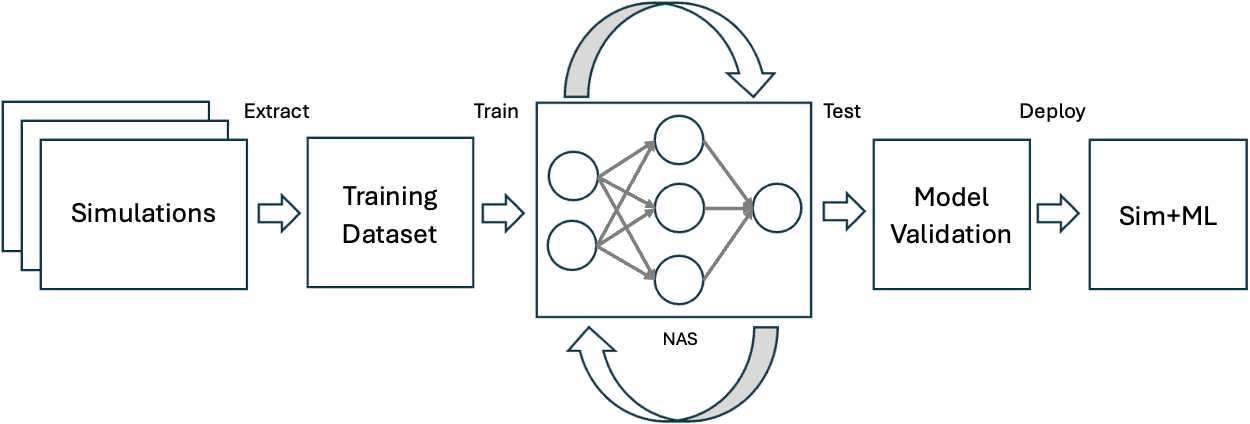
\includegraphics[width=0.8\linewidth]{images/workflow-surrogate-model.png}
    \caption{Machine-learned surrogate model training and deployment workflow \cite{brewer2023entropy}.}
    \label{fig:surrogate}
\end{figure}

\begin{figure}
    \centering
    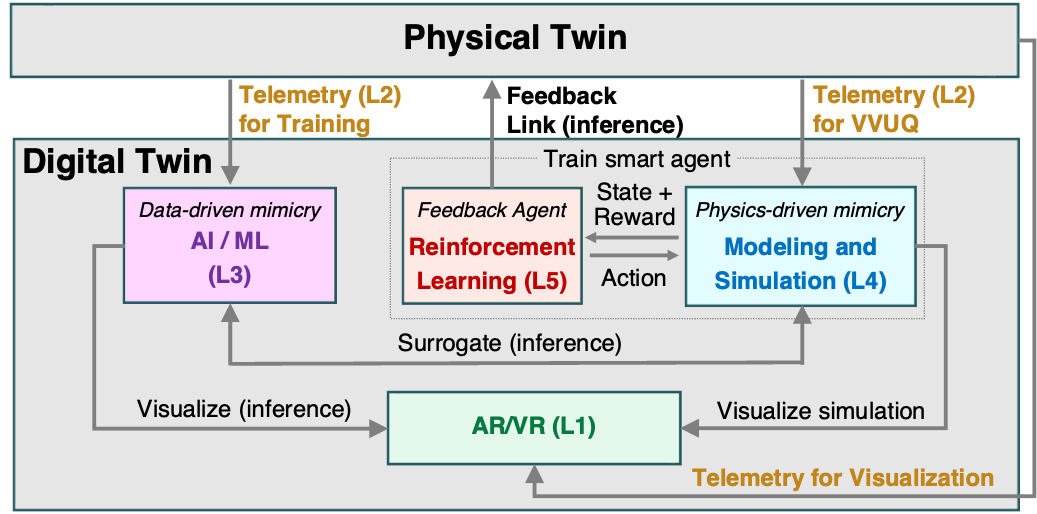
\includegraphics[width=0.8\linewidth]{images/workflow-digital-twin.png}
    \caption{Digital twin workflow \cite{brewer2024digital}.}
    \label{fig:dt}
\end{figure}


{\bf Shao} approaches workflow management from both the point of view of a domain scientist (with a particular emphasis on climate modeling) and a computer scientist investigating the emerging workflow paradigms and philosophies needed to combine AI/ML techniques with HPC-scale scientific simulations. In particular, most traditional numerical modeling operates as a pipeline with each stage focusing on the execution of a single application and the file system used to exchange data between stages. Ensemble-based modeling (often used in climate/weather) represents a horizontally scaled pipeline- each individual member ensemble may differ by the values of their tunable parameters and/or the initial/boundary conditions, but run independently of each other. HPC simulation and AI applications often require a more asynchronous computational paradigm with data exchange that occurs across loosely coupled components (i.e. processing elements transfer data through an intermediary). The SmartSim library provides well-maintained, open-source tooling that enables domain scientists to describe and execute their own complex workflows.

While originally designed for in-the-loop inference, increasingly the library has been used by users whose workflows apply AI techniques to ensembles of simulation (for example reinforcement learning). In general, these are characterized by a more complex set of outcomes/artifacts than traditional scientific modeling. For example, instead of just simulation data, workflow artifacts may include trained AI models or control schemes to be used in conjunction with digital/physical twins. 

{\bf Kirkpatrick} collaborates with workflow experts at several NSF and DOE-funded labs. Activities have included an invited keynote at a recent international workflows workshop, activities through GO FAIR US to promote the extension of the FAIR Principles for Workflows, and participation in other workshops \cite{kirkpatrick2023}. Her most recent scholarship includes a co-authored a section from a Dagstuhl seminar proceeding, ``Integrating HPC, AI, and Workflows for Scientific Data Analysis'' on sustainability in HPC and AI-driven scientific workflows \citep{badia2024integrating}.

To provide a better view of the various aspects of workflows we have organized them into a graph as shown in Figure \ref{F:graph-challanges}.




\section{Workflow Requirements}

In this section, we make some important observations that have a direct impact on workflow requirements particularly in the context of scientific computing done and their benchmarks at national laboratories and academia. These are largely distinguished from commercial workflows by the fundamental requirement to share results externally. Additionally, a strong trend towards open science and scientific reproducibility has also led to a push towards making the tools (e.g. simulation code, execution scripts, etc.) open as well.  

\subsection{Hardware Workflow requirements}\label{sec:hw-requirements}

In the US the HPC flagship computing resources have traditionally been offered by national scale computing centers, most notably the Department of Energy and the National Science Foundation. In addition, we see NASA, NSF ACCESS, NAIRR, and others augmenting such offers for specialized mission and scientific objective efforts serving particular communities. Others such as the DoD-related facilities are not available in general to the open science communities without restrictions, hence, we exclude them from our discussion. Other resources include commercial computing resources offered for example through cloud providers as part of hyper-scale computing centers.

Beyond these systems, we see additional regional or topical shared resources of medium scale, but also smaller scale systems that are available, for example, in many universities to allow direct access to HPC resources. Such tiered levels of HPC resources are necessary to serve the various communities that distinguish themselves as part of their computational needs based on topic and scale. These smaller systems also serve as an important on-ramp for training in preparation for accessing the leadership class or larger systems.  Due to this tiered approach, the European Union has defined three tiers as part of the Partnership for Advanced Computing in Europe (PRACE) \cite{www-prace,prace-fact} as follows {\bf Tier-0:} European centers with petaflop machines, {\bf Tier-1:} National centres, and {\bf Tier-2:} Regional centers.
  
However, when classifying the US resources we have used as part of our scientific and benchmark-oriented workflow activities, we suggest the use of a five-tiered model that classifies resources mostly by capacity:

\begin{itemize}
\item {\bf Capacity Tier-0:} Leadership Class machines with worldwide leading
  performance (Listed at the top of the Top 500 list). Such machines also include large specialized data file systems to allow serving the many computational nodes. Recently, such systems include a large number of GPUs. They are typically served by batch queuing systems and serve the most challenging scientific applications. An allocation request is typically needed to get access to such machines.
\item {\bf Capacity Tier-1:} Machines in the upper portion of the Top-500 list which may be part of National centers, Regional Centers, or Universities. Such systems are similar to those in Tier-0 but of significantly lower capabilities.
An allocation request is typically needed to get access to such machines.
\item {\bf Capacity Tier-2:} Machines whose performance is similar to machines
  in the rest of the Top 500 list. These machines are either smaller systems or if still operated older HPC machines that have been replaced by newer machines.
  An allocation request is typically needed to get access to such machines. In the case of universities, the HPC is shared based on internally set policies.
\item {\bf Capacity Tier-3:} Smaller scale HPC funded by a university or entity
  that are no longer listed in the Top500 list. Many universities have their own small clusters that are not as powerful but serve their individual communities or even labs. They may or may not run batch systems and at times use other software such as OpenStack, or more recently Kubernetes. 
\item {\bf Capacity Tier-4:} Privately owned machines supporting development
  and debugging. These are machines operated by individual researchers that may include powerful GPUs or CPUs, often performing faster than even those offered by their own universities. They provide an excellent cost-performance option for many researchers to develop and debug their programs quickly if the scale of the targeted application allows. These systems obviously are not targeting large parallel computing jobs. Although these machines do not typically represent an HPC machine as they are mostly single-node computers they can provide valuable input in performance expectations, development, and debugging.\footnote{See Section \ref{sec:data-requirements}.}
\end{itemize}

It is important to note that the top machines in the Top500 list dominate the capability tiers. 

This is evident as the Index Equilibrium is at about 7, that is the Rmax [TFlops/s] for
the first 7 resources of the list are equal to the sum of all other
493 resources, where Rmax is the maximal LINPACK performance achieved (see Figure \ref{fig:top500comparison}).


\begin{figure}[htb]
    \centering
    \begin{tabular}{cc}
        \vtop{\null\hbox{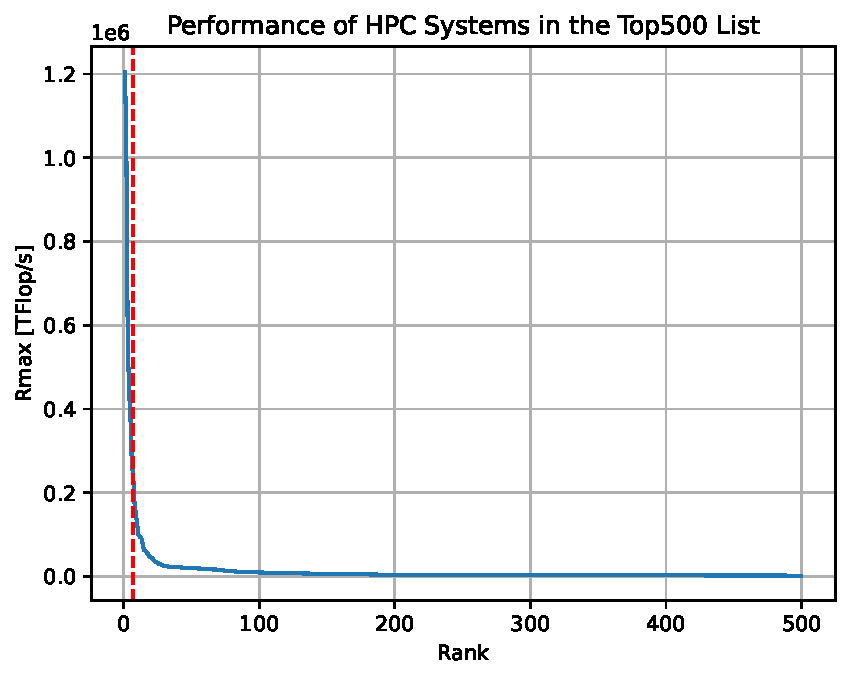
\includegraphics[width=0.45\textwidth]{images/top500/top500.pdf}}} &
        \vtop{\null\hbox{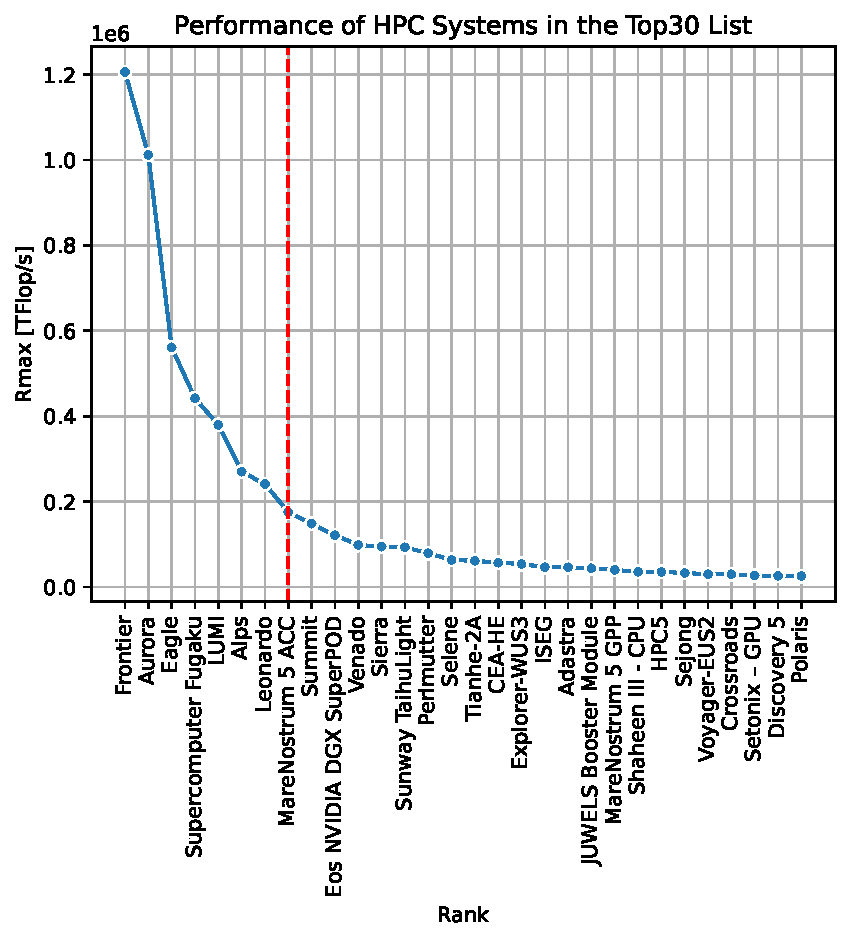
\includegraphics[width=0.45\textwidth]{images/top500/top30.pdf}}} \\
        {\bf a.} Top500. & {\bf b.} Top30. \\
    \end{tabular}
    
    \caption{Top500 List Comparison with the index equilibrium at about 7.}
    \label{fig:top500comparison}
\end{figure}


The latter tier has especially become important as it provides potentially significant computational power for developing a subset of scientific applications but lack integration in a shared user environment. Thus they are immediately available during the development and debugging cycles of the scientific workflow.

When accessing these resources they are mostly accessed through well-established queuing/batch systems to allow shared usage among the community accessing the resources. On larger systems especially when large scale experiments are needed this may result in significant runtime delays.

Scientific Workflows must be able to interface with such systems easily. Especially at the university level, we see however a significant complication in the use of such resources as often the machines integrate different heterogeneous resources into the batch system that makes intrinsic knowledge about the design and availability of specific resources necessary by its users. Furthermore, such systems may include older hardware, or have file systems not well integrated leading to a significant slowdown in the potential performance as we have discovered in \citep{las-frontiers-edu}. 

In general, all resources are accessible through remote access and is it well established that two concepts are used to access them. First, the use of SSH, and secondly, some systems also provide additional security through VPNs or 2-factor authentication (including RSA keys). Hence, if such systems are used in concert, we must be able to integrate with the various authentication mechanisms. Grids were supposed to solve this issue and at least for some US-based systems is continued in the use of inCommon \citep{incommon}. However, we found it is often easier to gather the authentication mechanisms and have the client easily authenticate to the systems to interface with them directly through their different keys. This is based on experience dating back even 30 years ago \cite{las-99-loosely}. Hence we refer to such workflow-integrated resources as heterogeneous loosely coupled resources.

To simplify access to several of them, we have developed additional libraries as part of cloudmesh in
support of the newer technologies going beyond the use of SSH. This includes the introduction of a split-VPN library and toolkit that allows accessing multiple VPNs dependent on which resource is being used and through which VPN this resource is being secured. Problematic in this case can however be if, for example, a university has decided not to universally support split VPN.

Alternatively, the Superfacility API \citep{Enders2020} proposes an externally accessible API (with authentication) that allows users to perform basic workflow tasks. With the correct requests, users can interact with the workload manager, upload/download files, and run shell commands. The primary downside to this approach is that it requires owners of the HPC platform to deploy and support this API.

Furthermore, in the Top500 100\% of the operating system family is Linux-based Thus
making the operating system family obvious. As also these days Windows
is supported either through Git Bash to emulate a Linux environment, shell scripts
can easily be ported to Windows as we have shown in cloudmesh, or
Windows Subsystem for Linux (WSL) can be used.  This allows us to restrict our development environment choices.



\tcbset{
    colback=yellow!20,
    colframe=yellow!50!black,
    title=Colored Box,
    breakable, % Makes the box content breakable across pages
}

\newenvironment{BOX}[1][title]
{
    \ifx\homepath\overleafhome
        \bigskip
        \begin{quote}
        \begin{mdframed}[hidealllines=true,backgroundcolor=yellow!20]
        \hline
        {\bf #1}
    \else
        \begin{tcolorbox}[title=#1]
    \fi
}
{
    \ifx\homepath\overleafhome
        \hline
        \end{mdframed}
        \end{quote}
    \else
        \end{tcolorbox}
    \fi
}

\begin{BOX}[Implications from Section \ref{sec:hw-requirements} Hardware requirements]

\begin{itemize}
\item {\bf Hardware at scale:} {\it The hardware that we need to
    support includes a wide range of large HPC systems down to the individual researcher's computer.}
\item {\bf Interface to workload managers:} {\it As different systems
    have different workload managers such as SLURM, LSF, SSH, and
    others the workflow system must be expandable and allow easy
    integration of workload managers by the community.}  
\item {\bf Minimal support for access:} {\it Although it is not
    necessary to support a fully federated resource infrastructure,
    client-based workflows must support the integration of
    heterogeneous resources with potentially different workload
    managers. Access could be supported through multiple keys or
    services that are specifically set up by the user to allow
    interfacing with the hardware.}
\item {\bf Minimal support for virtualization in the cloud:} {\it Although we
    previously spent a lot of time interfacing with virtualized
    resources and cloud-based resources, we recently have shifted our
    focus on the more traditional approach to interface with queueing
    managers. This is motivated by the fact that many of the
    most complex state-of-the-art projects are conducted on the most
    capable machines (the first 7 machines in the Top500 provide the
    same compute power as all the rest of the 500).}
\item {\bf Batch access and direct access:} {\it As many of the
    workload managers are batch queuing systems we need to support
    them in general. However, as we also have access to machines that
    may not be controlled by batch queues, we need to be able to
    potentially simulate such batch queues, or provide mechanisms to
    install them so that such resources can simulate the same
    interfaces as those provided by HPC centers.}
 \item {\bf Cloud HPC resources:} {\it Most recently several cloud
     vendors are also supporting the provisioning of HPC resources,
     but the complexity of managing them is beyond those present by the
     typical application users. Workflow systems should support to
     more easily provision of such HPC resources so they can be readily
     integrated into the scientific research and benchmark efforts.}
 \item {\bf Container and virtual machine support:} {\it Obviously we
     have learned that the use of virtual machines in clouds can be of
     benefit to create portable workflows utilizing the. The same is
     valid for containers. Thus a potent workflow system ought to
     support both virtual machines and containers. In the case of
     containers, this included docker, with Kubernetes and especially Apptainer as the latter
     dominates virtualization activities on HPC machines due to heightened security aspects
     isolating the runtime environment. }
  \end{itemize}
\end{BOX}

\subsection{User Requirements}
\label{sec:user-requirements}

To identify the user requirements we have to first ask ourselves who are the users. Throughout our rich experience, we encountered the following user groups:

\begin{itemize}
    \item {\bf Application users} are users with focus on application usage. Often they are supported by Graphical User Interfaces, Gateways, or even customized application-specific frameworks. In many cases, the complex workflows to utilize sophisticated cyberinfrastructure including hardware and software is hidden from the users. However, this may come with the problem that such users may not adequately access what cost a particular workflow causes. Thus the support of such users not only needs to be user friendly but also project in easy-to-understand terms the expected runtime costs for experiments conducted with them. This may include not only the dollar cost but other factors such as availability, wait time, and energy costs.
    \item {\bf Application Scripters} are users that may not have GUIs or Gateways available or even prefer to use scripts to formulate their experiments. This may include shell scripts, or programming languages such as Python to coordinate the experiments. The requirements for such users include that the scripting must be easy enough so that it still allows the application to be the main focus of their work. In some cases, the result of such scripts are templates that through reuse can accelerate the repeated execution of experiments. When using HPC systems users typically have to learn how to use the batch queuing system, as well as have minimal understanding of the command shell. 
    \item {\bf Application developers} are developing specialized applications as part of their scientific workflows. They either develop the workflows from scratch as part of the regular programming or reuse libraries that interface either with the application domain or the cyberinfrastructure so that through reuse the experiments they target can be simplified through sophisticated but easy-to-use APIs, libraries, experiment management workflow components that coordinate one or multiple experiments. It is important that the libraries that are developed for this community can be integrated in some fashion into the preferred programming language, or framework. This may go beyond the availability of Python frameworks that are very popular with AI experiments. 
    \item {\bf DevOps Engineers} tasks include the management of a software development life cycle and enabling the integration of cyberinfrastructure to allow workflows that integrate automated provisioning, testing, and release management. They can be essential in the better utilization of the infrastructure in general but also support large-scale experiments that are these days more common while utilizing large-scale cyberinfrastructure. Experiment workflows thus need not only be able to be defined by application users for large-scale HPC but it is advantageous to consult with DevOps Engineers to fine-tune experiments before they are placed on the infrastructure or are refined throughout their lifetime. A whole set of tools have been developed in support of DevOps which we will not get into further as it deserves its own paper.
    \item {\bf System Administrators and Support Staff} are supporting experiments while keeping up the systems designed for a user community. They will provide support and help to any users utilizing their infrastructure. In many cases, application users do not need or access DevOps Engineers but interface directly with the System Administrator to define strategies to utilize the infrastructure for their experiments. In all organizations we used HPC resources for experiments dedicated support was available to address questions on how to improve the runtime experiments as well as application performance improvements.
    \item {\bf Organization and Funding agencies} are an often overlooked part of the scientific experiment workflow. They provide in many cases access to the often costly infrastructure and need to be informed how they are used. This may include not only an overall breakdown for the entire organization, but it can also help the individual experimenter to understand their own demands placed on computing resources (see \citep{las-15-tas}). 
\end{itemize}

From this diverse set of users that we encounter in support of experiments, it is obvious that the requirements vary by user group. While for example, the application user is satisfied with a high level interface an application developer and scientific researcher may need access to much more sophisticated tools and libraries. In many cases, they could also benefit from a standardization of libraries that supports their and other researchers' experiments even across domains. The education of the users may play a very important role. While we have seen in some projects users have been educated by system staff, the users as well as the system staff may not have known tools that simplify certain processes in the experiment management workflow. For example, we did a test where a group of graduate and undergraduate students struggled over six months to develop a reproducible FAIR-based experiment while just using batch scripts, while they could have chosen one of our workflow systems that specifically addresses this issue which a much more easy to use and powerful solution provided by the cloudmesh experiment executor or SmartSim. In the case of the experiment executor, we showed that the same experiment workflow set up by the team of 4 students (including 2 graduate students) working on this for six months could be executed by a single undergraduate student in a matter of a day. Not only that, the results produced by the single student were reproducible and scientifically sound as they were verified independently.

One of the most important lessons we obtained from it was that experiment workflows require a proper framework to be able to reproduce the experiment. This includes experiment parameters for the application and the infrastructure, as well as an easy-to-understand mechanism to record and catalog data products created by not only one but potentially many thousands or hundreds of thousands of experiments. This is based on our own experience when an experiment needed to be repeated to identify issues with the data, or to conduct quality or performance improvements as part of benchmarking the experiments. This also includes the fact that such experiments must be designed in a portable fashion so they can be executed potentially on different infrastructures for performance and even accuracy comparisons (in case different architectures are used).


\begin{BOX}[Implications from Section \ref{sec:user-requirements} user requirements]

\begin{itemize}

\item {\bf Wide Variety of Users:} {\it To support the wide variety of users experiment management needs to be available from the lowest to the highest level of interfaces targeting the specifics of the user community. This has a significant impact on the software in support of these communities which we explain in the next section.}
\item {\bf Ease of Use:} {\it In order for the user community to utilize experiment management it is important that whatever tool and software is supported it can easily be used by the targeted user community.}
\item {\bf Experiment Automation:} {\it Users strive for replication of their experiments. This includes experiments that can be replicated by different users, but also experiments that can be replicated on different hardware.}
\item {\bf Experiment Reporting:} {\it As experiments are recorded at a particular time under a selection of software and hardware utilization, it is important that results encompass reporting of the environment. This will help the reproducibility of the experiment and if the underlying system has changed the repetition of the experiments with minimal changes.}
\item {\bf Portability:} {\it Users that conduct benchmark experiments also require portability which allows them to compare and contrast different experiment setups on different systems.}
\item {\bf Cost Considerations:} {\it One important factor in conducting benchmark experiment workflows is the ability to understand cost considerations prior to running a large-scale or time-consuming experiment. Having the ability to scale and predict performances from a small scale to the target scale is an important need. Tools and software should be provided that assist in this often complex endeavor.}

\end{itemize}
    
\end{BOX}

\subsection{Software Requirements}
\label{sec:sw-requirements}

In Figure \ref{F:graph-challanges} we have already listed many of the topics that influence the software design and requirements. Due to the diverse user community, a one-fits-all solution can not be applied and the solution must be addressing in particular the specific user communities.

For this reason, we distinguish important abstractions to formulate experiment workflows. This includes in particular arrays and loops of experiments iterating over hyperparameters or specific machine configurations to be provisioned or used. 
Although DAGs allow us to coordinate experiments also, we found that in many cases where iterations are called for equivalent specifications can be more easily formulated with loops and arrays. This insight was already available in our earlier work where we allowed iterations and dynamically changing workflow graphs \citep{las07-workflow} in addition to DAGs. The functionality ought to be exposed on various levels. This includes availability in the queuing system (which many of them provide), the availability as API to integrate in convenient fashion functionality into frameworks or even programming languages, or providing high-level abstractions such as YAML formulations that allow the definition of iterations or DAGs in easy fashion within easy to understand formulations. The latter is a reformulation of our earliest work that included specifications on a higher level in specialized formats \citep{las-96-ecwmf}  or XML \citep{las07-workflow}, but are now done for example by using YAML and JSON replacing template to formulate high-level templates to start experiments \citep{cloudmesh-cc,cloudmask-ee}.

Through the availability of low-level and high-level functionality that is exposed through APIs and a convention based on for example an enhanced experiment workflow description leveraging YAML, the functionality can through software engineering incorporated in any framework or application. 

As we specifically target the combination of hyperparameters (or just parameters when not using AI) as well as introducing parameterized infrastructure we truly address experiment management through the combination of all these factors.

This allows the the support of the experiment workflow including data pre-staging, computational calculations
checkpointing/restoring, result recording, and backup.

Through the availability of these functionalities on various abstraction levels while leveraging the same backbends we can flexibly integrate the appropriate solution in the various levels without necessarily having to address or repeat them throughout the software stack. One way of dealing with integration into other frameworks is to provide interfaces for example in OpenAPI. This will allow in many cases a sufficiently detailed integration in other languages also through the wide support of OpenAPI. However, due to the dominant use of Python in academia as part of newer developments, we promote the use of a native Python API. for our work. This has the advantage that many built-in libraries and tools can be leveraged to simplify the development of integrated workflows. Obviously we also can leverage the language support for loops and existing libraries to support graphs which we have demonstrated successfully in \citep{cloudmesh-cc}.

Considering that superuser access to HPC platforms is often limited to a very small subset of support staff, software must be able to be run with basic user privileges. Software designed for containers and/or for deployment in the cloud tends to assume that they have the ability to register system-level services and/or kernel-level access. This is not the case on many of the machines available to the academic public. As such, some container technologies commonplace in the cloud are simply not available on major HPC platforms.

\subsubsection{Software License Requirements.} 

Cloudmesh initially used MongoDB for managing a cached version of its infrastructure. This however had early issues as the documentation and installation instructions for Windows at the time were insufficient and not well documented. Hence, we spend uneccesarry time and wrote our own better installation workflow for it. Unfortunately MongoDB changed in 2018 the license and it was impossible for us to continue using MongoDB.  At this time we completely rewrote cloudmesh to use its own internal YAML database based on Python. This allowed 
a much easier pip only install and simplified the setup of cloudmesh drastically. This was also the main issue brought forward by our users, ``eliminate MongoDB dependencies.'' 

Recently SmartSim ran into a similar  problem as it could not distribute Redis on which it currently depends with a precompiled version including containers. Often Alternatives are not available till such license changes have been made and introduce considerable inconvenience to the existing dependent projects. Currently, an alternative to Redis would be KeyDB  \citep{keydb}. 

However, as a lesson {\em it should be avoided to rely on nonpublic domain software that provides license restrictions.} Even recently it was annonced that conda is no longer free to use for organizations with more then 200 employees, which essentially means any university and research lab. As it is used often in AI workflows, now pathways have to be found. Luckily, cloudmesh and SmartSimn do not depend on conda. 

At the same time, the software to manage the workflows should be distributed under a well-known and established open-source license allowing others to also easily contribute. In case of Cloudmesh we have chosen Apache 2.0 due to our good experience for over a decade within many software projects.
SmartSim is distributed under the BSD-2-Clause license.


\subsection{Runtime Requirements}

Besides typical runtime requirements such as speed and access to the available hardware through APIs, we especially note that often we need to address policy-based restrictions to the resources. This for example includes addressing queueing system policy restrictions set up by the organization and managed by the administrators. Although such restrictions could be changed, they are often not scalable as they need to be changed back. However, in many cases reformulating the experiment workflow can overcome such restrictions. For example, a job that is terminated due to exceeding time restrictions could be split into multiple jobs while allowing checkpointing at the end of the individual jobs and restarting them into the next phase can help. In other cases instead of creating a loop over all possible calculations needed to conduct the overall experiment, submitting multiple jobs with the experiments split up between them can be used. While assuring that the results are being stored in a coordinated fashion following the FAIR principle the analysis of the final result while combining the results of the many individual experiments can be split up and if often preferred as for example such experiment management can even deal with outages of the resources. Another example is where a resource allows the utilization of thousands of CPUs or GPUS, but only for a small amount of time. In such cases, the application user ought to be encouraged to parallelize their algorithms and the experiment framework needs to support such a modality. This, however, is outside of the scope of our work and needs to be addressed by the application developers. Small-scale runtime experiments could be used to project how the runtime or the design of an algorithm is impacted by such queueing policies.
Furthermore, we note that such policies differ widely between HPC systems and need to be integrated into the planning of a heterogeneous experiment across resources. Obviously, the availability of time and space limits at runtime that could be queried dynamically can help improve the deployment of dynamic experiments that deal with the limits if they arise. Guidelines and APIs to checkpoint an application will be of importance. However, although automatic checkpointing is desired, for many applications only a fraction of data is needed and not the entire state of the running application. Therefore it is best to identify data that is needed in consecutive runs and only checkpoint those.


\subsection{Security Requirements}

The desire to execute benchmark workflows on multiple HPC resources to compare them will bring up the topic of federated resources using the same security context. However, although they could be achieved in organizations such as DOE, we will always have resources that are outside a single federated organization. This is not only due to the independence of many research organizations and universities but also due to policies in place by the countries in which they operate. Hence, it is important that other means are used to allow using resources from a wide variety of organizations from which we know that federation can not be achieved.

One way of comparing results is to simply establish a results repository as spearheaded by MLCommons to which vetted members submit their results. In other cases, results may be produced by different teams that have access to different resources. In each of these cases, the underlying result is structured in a particular fashion so that they can be contributed in a shared file system or repository. As part of this, the results must be structured in a uniform way. We have devised such a structure as part of our work in which we contribute results in a tree organized by organization, resource, application, and experiment. As the application benchmark workflow results are uniformly formatted, they can easily merged and analyzed across organizations and resources. 

To allow maximal progress with minimal effort we did not further explore the use of more formal federation capabilities, but rather focus on how distributed experiments can be merged in a federated result repository. This is done typically by a lead organization and results are loosely contributed to the organization's case (such as demonstrated by MLCommons). This also naturally allows the contribution of results from the same organization that have been gathered by multiple users. This may be useful in case policy restrictions restrict the execution of a large number of experiments needed to complete the overall benchmark.

However, in some cases, we had access to multiple resources ourselves spanning DOE, NSF, and University resources. In these cases, we observed that all resources could be accessed through SSH and heterogeneous experiments using a variety of resources could be easily formulated. However, we encountered on the university level a particular obstacle as several used their own VPN not allowing the use of multiple VPNs at the same time. We overcame this obstacle by considering using splitVPN and implemented an easy-to-use API and command line tool based on OpenVPN while consulting with the developers of OpenVPN. 

Obviously, when using cloud resources such as HPC resources provided by major cloud providers, federated security becomes even more complex and our strategy to stay within the cloud based security context for such resources is at this time not  simple mechanism to integrate such resources in a wider benchmark effort.


\subsection{Data Management Requirements}
\label{sec:data-requirements}

In order to support data benchmark requirements we need to consider the wide variety of data needs served by the benchmarks. This includes statically generated data which may not involve any data storage, and reaches hundreds of petabytes for the training of for example large language models. As the full training as part of a benchmark is out of scope for the benchmark initiative, smaller data sets are used. 
We see in other cases the uses of a few files, but in other cases a plethora of files incorporated into an application benchmark. The inclusion of such data can reveal shortcomings of the hardware design, leading to potential issues that despite the availability of modern CPUs and GPUs the file system is not designed to leverage them efficiently as the workflow to utilize them can not keep them busy and the data management becomes a bottleneck. We have shown recently that at a university cluster, this was the case. Thus benchmarks should not only project the potential of the sheer computational power of a system but also integrate the data I/O performance.

% \TODO{this is duplicated in tier section}

%%%%%%%%%%%%%%%%%%%%%%%%%%%%%%%%%%%%%%%%%%%%%%%%%%%%%%%%%%%%%%%%%%%%%%%%%%%%%%%
\subsection{Recent Application Experiment Workflow Requirements}
%%%%%%%%%%%%%%%%%%%%%%%%%%%%%%%%%%%%%%%%%%%%%%%%%%%%%%%%%%%%%%%%%%%%%%%%%%%%%%%
\label{sec:application}

We have gained our requirements from a large number of applications from various domains over the last 30 years. However, we like to focus here on more recent applications that we are trying to integrate into our experiment workflow activities. This not only includes the effort on digital twins as described earlier but also on ocean climate modeling with MOM6 and on the development of an Open Model Surrogate Inference (OSMI) benchmark. We focus here on the latter and describe it in more detail.

%%%%%%%%%%%%%%%%%%%%%%%%%%%%%%%%%%%%%%%%%%%%%%%%%%%%%%%%%%%%%%%%%%%%%%%%%%%%%%%
\subsubsection{OSMI}
%%%%%%%%%%%%%%%%%%%%%%%%%%%%%%%%%%%%%%%%%%%%%%%%%%%%%%%%%%%%%%%%%%%%%%%%%%%%%%%

Most AI workflows on HPC can be categorized into six different execution motifs: Steering, Multistage Pipeline, Inverse Design, Digital Replica, Distributed Models, and Adaptive Training \cite{brewer2024ai}. One component that shows up across multiple motifs is machine-learned surrogate models. Such models typically are used in hybrid ModSim/AI workflows, where traditional simulations are used for a large part of the workflow, and then particular aspects of the simulation, such as a turbulence or radiation model, are replaced by digital surrogates, e.g., \cite{partee2022using, martinez2022roam, bhushan2023assessment}. Because of the challenges of integrating the simulations with the AI model in a highly scalable manner, developing a benchmark was necessary to assess the performance of various configurations. Initial developments of a surrogate model benchmark, called ``OsmiBench'', were studied by Brewer et al. \cite{brewer2021production}. The studies showed that using a separate load balancer on each compute node, which round-robins the inference requests across multiple GPUs on the node, and also using the maximum batch size that the GPU memory allows yields optimal inference performance. This study was followed by a secondary investigation by Boyer et al. \cite{boyer2022scalable}, which investigated performance implications of the full coupling between the surrogate inference and the simulation code, and showed that using a concurrency level of two batch inference requests was optimal. 

The Open Surrogate Model Inference (OSMI) benchmark was developed as an open-source community benchmark founded upon these principles. The architecture of OSMI is shown in Fig. \ref{fig:osmi}. The benchmark supports either TensorFlow or SmartSim/PyTorch-based frameworks as shown in Table \ref{tab:osmi}. Inference requests are initiated from within the simulation using a client API call (e.g., SmartRedis or gRPC API), the requests are then sent to a load balancer (e.g., HAProxy), which distributes the requests in a round-robin fashion to multiple inference servers, each bound to a single GPU. Benchmark timings are able to be measured at multiple places in the architecture, but the primary measurement of interest is how long it takes from the time an inference request is initiated from the simulation until the response is returned back to it. As opposed to chip-level benchmarks such as MLPerf \cite{reddi2020mlperf}, OSMI is able the measure system-level performance, which includes the performance of the CPU, GPU, network, and interconnect (IC), giving a holistic performance representation of the system. This same approach was used to benchmark a wide range of HPC systems, revealing significant performance differences between seemingly similar machines, often due to factors such as different interconnect performance \cite{brewer2020inference}.

\begin{figure}[t]
    \centering
    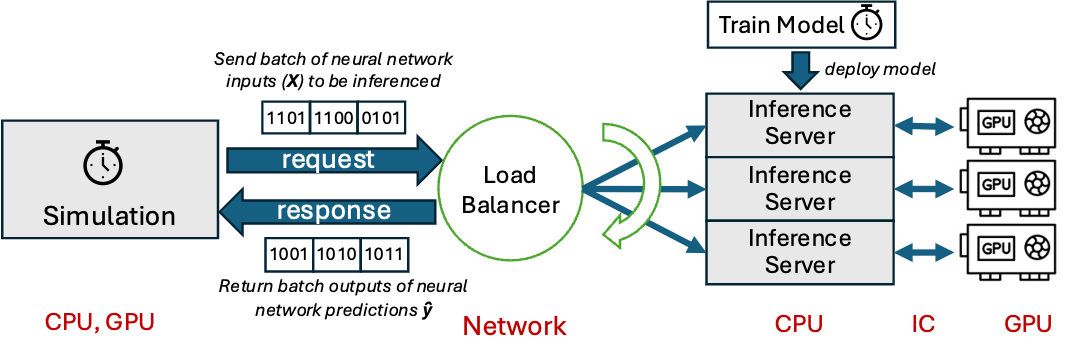
\includegraphics[width=\linewidth]{images/osmi_arch.png}
    \caption{Architecture of OSMI benchmark.}
    \label{fig:osmi}
\end{figure}

\begin{table}[t]
\centering
\renewcommand{\arraystretch}{1.5}
\begin{tabular}{llll}
\hline
\textbf{AI framework} & \textbf{Inference server} & \textbf{Client API} & \textbf{Protocol} \\ \hline
TensorFlow & TF Serving  & TF Serving API  & gRPC  \\
PyTorch    & RedisAI     & SmartRedis      & RESP  \\ \hline
\end{tabular}
\caption{OSMI-supported AI frameworks.}
\label{tab:osmi}
\end{table}

\begin{BOX}[Requirements implied by the OSMI benchmark]
The immediate requirements we gather from such a complex experiment workflow are (a) the interplay between large computational components executed on GPUs that are interwoven with the overall execution in an iterative simulation executed on multiple servers (b) the scheduling of thousands of independent calculations executed on the GPUs while hyperparameters and data sets need to be feed to the executing GPUs, and (c) the gathering of the results in a mathematically sound dataset, and (d) the execution of such a workflow on different architectures to showcase the wide variety of performance differences while configuring the workflow specifically for the various target machines.
\end{BOX}


%%%%%%%%%%%%%%%%%%%%%%%%%%%%%%%%%%%%%%%%%%%%%%%%%%%%%%%%%%%%%%%%%%%%%%%%%%%%%%%
\subsubsection{Cyclic Experiment Execution} \label{subsubsection:cyclic}
%%%%%%%%%%%%%%%%%%%%%%%%%%%%%%%%%%%%%%%%%%%%%%%%%%%%%%%%%%%%%%%%%%%%%%%%%%%%%%%

Workflow execution has typically focused on workflows that can be represented by a pipeline or more generally a directed acyclic graph (cycles with predefined loop limits can be unrolled). Many solutions exist to execute and monitor these types of workflows (e.g. Parsl or Maestro). In both these cases, the execution is deterministic.

Other types of workflows, becoming more popular in scientific applications, involve branches or criteria-based loops, thus violating the fundamental assumptions of a DAG. One common application is automatic parameter estimation.  For example in \citep{Maric2024OpenFOAM}, a Bayesian optimizer is applied to an OpenFOAM computational fluid dynamics case. The optimizer at every iteration generates candidate parameter sets which are then used to launch new cases. The output from those cases is then ingested by the optimizer for the next iteration. As is typical of optimization problems, this cycle ends when either the loss function converges, stalls, or reaches a certain number of optimizations.

Reinforcement learning is another type of workflow that involves non-cyclic and potentially branching workflow execution. In \citep{Font2024}, an ML model is used to control the behavior of a turbulent flow surrounding a rising bubble. The ML model is able to modify the flow by controlling actuators.  The RL model deploys multiple agents in various environments to explore and refine the optimal actions. Similarly, \citep{Kurz2022} train a surrogate model of turbulence using an RL framework. The agent predicts an eddy viscosity where the RL model is incentivized to match the energy spectra in a turbulence-resolving model. As in \citep{Font24}, the scientific simulation is used as an environment to evaluate the agents' strategies. In both these cases, the need to continue to iterate and test requires dynamic configuration and execution where the number of cycles is not known a priori.



%%%%%%%%%%%%%%%%%%%%%%%%%%%%%%%%%%%%%%%%%%%%%%%%%%%%%%%%%%%%%%%%%%%%%%%%%%%%%%%
\subsection{Requirements for Benchmark Carpentry}
%%%%%%%%%%%%%%%%%%%%%%%%%%%%%%%%%%%%%%%%%%%%%%%%%%%%%%%%%%%%%%%%%%%%%%%%%%%%%%%
\label{sec:carpentry}

In \citep{las-frontiers-edu} we introduced the concept of benchmark carpentry in relationship to educational activities as we believe that based on our own experience this topic is much needed but is not adequately addressed. 

When designing benchmarks, it is important to think of the results as experiment data, rather than just an answer to a performance question. 
This implies that we not only run a particularly designed benchmark with fixed data but that the data itself has a significant impact on the benchmark and needs to be considered as a benchmark variable.

Organizing data for later reuse also allows for later application of machine learning to uncover additional insights that can lead to further optimization, e.g., subtle performance gains related to specific software and hardware device combinations. 
This leads to a potential complication in organizing and interpreting the data. We need to make sure our benchmarks are structured in an organized fashion so this is avoided.

The FAIR principles provide a framework for aligning research outputs. FAIR is an acronym with 15 underlying principles that relate to Findability, Accessibility, Interoperability, and Reusability (FAIR) \citep{wilkinson2016fair}. More specifically, the FAIR Principles call for the use of well-described, standardized metadata, clear licensing and usage information, open or freely available protocols and methods for access, and the use of globally unique identifiers. The actual implementation of the FAIR Principles varies by domain, data architecture, and resources available to sustain data management practices and infrastructure \citep{jacobsen2020fair}.

In the case of this work, several practices were identified that relate to making HPC benchmark results more FAIR\citep{kirkpatrick2024}. These include ensuring controlled vocabularies are used when describing system information. Where these are not available, it is preferable for the software, such as cloudmesh, to extract information from other sources, such as system configuration, libraries, or registry settings, especially over the use of free-form text. Ideally, globally unique identifiers would be assigned to each benchmark output. Other implementations of FAIR can include writing provenance information about how the benchmark was created in the results file. The FAIR Principles in this work are also exemplified in structured abstraction, e.g., the use of YAML, the use of standardization, e.g., NIST standards, and (machine) accessibility via an API. 

From the efforts surrounding cloudmesh and SmartSim, we have learned we must support as part of the benchmark carpentry as defined in \citep{las-frontiers-edu} also tasks related to  (a) installing software, (b) reserving compute resources for exclusive use, (c) preparing experiments (potentially using a large number of batch jobs) and executing them, (d) evaluating and validating the resulting performance including computational power of CPUs, GPUs, data I/O, networking, and energy, (e) record the results in a uniform format so that comparisons can be made (f) and submit results to the community to allow others to contribute, either through publications or efforts such as promoted by MLCommons. All of them should ideally be integrated in a well-defined mechanism allowing to support FAIR.


%%%%%%%%%%%%%%%%%%%%%%%%%%%%%%%%%%%%%%%%%%%%%%%%%%%%%%%%%%%%%%%%%%%%%%%%%%%%%%%
\section{Experiment Execution Templates}
%%%%%%%%%%%%%%%%%%%%%%%%%%%%%%%%%%%%%%%%%%%%%%%%%%%%%%%%%%%%%%%%%%%%%%%%%%%%%%%
\label{sec:templates}

From the requirements we identified, which were derived from applying experiment workflows to actual applications, we learned that one of the best mechanisms to deal with the variety of infrastructure and their underlying software infrastructure and hardware resources, which change over time, is to start thinking about providing ``templates'' specifically designed for resources and application that can be modified and adapted to either address the changing infrastructure or used to port new applications. For such templates to be defined we need to specifically consider HPC, Hyperscalar, federated, and cloud resources.

%%%%%%%%%%%%%%%%%%%%%%%%%%%%%%%%%%%%%%%%%%%%%%%%%%%%%%%%%%%%%%%%%%%%%%%%%%%%%%%
\subsection{Experiment Execution on High Performance Computers}
%%%%%%%%%%%%%%%%%%%%%%%%%%%%%%%%%%%%%%%%%%%%%%%%%%%%%%%%%%%%%%%%%%%%%%%%%%%%%%%

In general, users on HPC platforms operate in a computing environment with fixed computational resources and storage which. This strongly influences the types of experiments that are executed on these platforms which are generally characterized by inelastic workloads with pre-defined execution.

In particular, users often operate within fixed size allocations (e.g. users have N node-hours with a pre-specified end date). Executing experiments on traditional HPC platforms is characterized by submitting batch jobs to the workload manager (e.g. SLURM or PBS). Additionally, because the amount of work is primarily static, large amounts of resources are allocated for long blocks of time (hours, days, or weeks). Long-running tasks on login nodes are generally discouraged although more recent HPC platforms include the concept of `workflow' nodes that can be used to deploy long-running. This leads to experiment execution following pipeline-like workflows with each batch job submitting a new batch job to execute the next stage.

HPC users also tend to assume that data is stored locally and in a persistent state. This allows experiment execution to use the file system as a way to swap data and/or store the state between submissions of batch jobs. Tape archives are used for long-term storage, however by its nature the time to retrieve large amounts of data can be cumbersome.

Comparatively speaking, most applications run on baremetal, i.e. outside of a container. The main advantage of containers, providing a portable environment, is less of an issue on HPC platforms which tend to retain the same hardware over the lifetime of the machine and whose software libraries are updated relatively infrequently.

In many cases templates to formulate batch jobs are available from the organization hosting the HPC resource.

%%%%%%%%%%%%%%%%%%%%%%%%%%%%%%%%%%%%%%%%%%%%%%%%%%%%%%%%%%%%%%%%%%%%%%%%%%%%%%%
\subsection{Experiment Execution on Hyperscaler Resources}
%%%%%%%%%%%%%%%%%%%%%%%%%%%%%%%%%%%%%%%%%%%%%%%%%%%%%%%%%%%%%%%%%%%%%%%%%%%%%%%

The increasing availability of resources in the cloud has led to an increased interest in deploying traditional HPC workloads on hyperscaled resources. These platforms have traditionally been optimized for web applications where elasticity of resources is paramount to adapt to dynamically changing workloads.  With the increasing use of the cloud for machine-learning tasks, hardware that was typically only available on HPC platforms (e.g. high-bandwidth, low-latency interconnects) are now commonplace. In contrast to traditional HPC, users have instant access to an (apparently) unlimited amount of computational resources and storage.

The elasticity of resources leads to experiment execution paradigms that are driven by service-oriented architectures. This includes spawning multiple workers for each service that are ephemeral, often completing a small unit of work before ending. Applications are loosely coupled with communication and requests are handled through APIs instead of communicating directly with each other.  In contrast to bare-metal HPC, containers are a fundamental requirement to create customized environments that can be very quickly deployed and scaled onto a new set of resources. Jobs are usually measured on the order of minutes or seconds.

Templates to use such resources are often provided as sample applications.

%%%%%%%%%%%%%%%%%%%%%%%%%%%%%%%%%%%%%%%%%%%%%%%%%%%%%%%%%%%%%%%%%%%%%%%%%%%%%%%
\subsection{Federated Experiment Execution}
%%%%%%%%%%%%%%%%%%%%%%%%%%%%%%%%%%%%%%%%%%%%%%%%%%%%%%%%%%%%%%%%%%%%%%%%%%%%%%%

Federated computing is a larger scale of computing that takes advantage of resources across multiple HPC platforms. This might either to perform computations that are larger than the resources available on a single HPC platform and/or to support applications with heterogeneous hardware requirements (e.g. a part of the application may be performant on GPU whereas another part might be better suited for many-core CPUs). 

Workflow templaes such as provided in cloudmesh to showcase multiple resource utilization can easily used and if needed adapted to serve federated experiment execution. 

%%%%%%%%%%%%%%%%%%%%%%%%%%%%%%%%%%%%%%%%%%%%%%%%%%%%%%%%%%%%%%%%%%%%%%%%%%%%%%%
\subsection{Experiment Execution on Clouds}
%%%%%%%%%%%%%%%%%%%%%%%%%%%%%%%%%%%%%%%%%%%%%%%%%%%%%%%%%%%%%%%%%%%%%%%%%%%%%%%

The CoGKits for Java and Python were the predecessors to cloudmesh. While those tools focused on Grid computing interfaces for the various Grid toolkits. Cloudmesh provided the opportunity to shift its focus to services offered by cloud computing including Azure, AWS, Google, OpenStack clouds, and Chameleon Cloud via OpenStack. Here cloudmesh focused on the creation of a very simple mechanism to start compute resources uniformly on the various clouds while providing templates that offer similar capabilities across them. As such workflows could be created that allowed switching easily between virtual machines. This is achieved by the cloudmesh command line and command shell that prior to any other tool allowed integrating and switching between clouds easily. Thus to start a VM on AWS, and then one on Azure one could simply say

\begin{verbatim}
  cms set cloud=aws
  cms vm start
  cms set cloud=azures
  cms vm start
  cms vm start --cloud=google
\end{verbatim}

Build-in defaults can be aligned so that the virtual machines operating on the various clouds are similar.
Cloudmesh was the first tool that promoted a setup of cloud credentials in YAML files that were used to start ``templated'' virtual machines with default parameters provided by these templates. Only later were similar capabilities integrated in, for example,  OpenStack. Thus we can support cloud-based workflows

\begin{itemize}
    \item on one or multiple clouds
    \item cloud agnostic workflows
    \item adding easily new clouds into the workflows by integrating access points
    \item allowing the integration of new clouds and their virtual machine access protocols
\end{itemize}

As clouds have recently also integrated containers and serverless computing we have prototyped the ability to stand up Kubernetes clusters (in AWS for example). As setting up such clusters is a task that is beyond the capabilities of scientists we prototyped an easy way to set them up including default security and network capabilities. The integration into cloudmesh is conducted through the cloudmesh plugin mechanism that ads dynamically this capability with a simple pip install.

Most recently a shift in scientific computing has taken place that emphasizes the use of GPU compute resources. For this reason, AWS has added the ability to bootstrap in the cloud parallel clusters including their control through SLURM. Obviously, this could also be leveraged by a scientist who may not have a supercomputer at their facility or wants to conduct an HPC workload in the cloud. However, the configuration and setup is something most scientists do not want to be bothered with. Their goal is the access to the compute resources. Our cloud cluster plugin to cloudmesh therefore contains the ability to deploy a cloud cluster with or without GPUs, as well as the size of the working node with the help of a single command to which we specify such things as the name of the cluster, how many nodes, and if and which GPUs should be used. Obviously, that can all be configured through AWS cloud formation, however, the setup and the configuration parameters are too complex to just support this general workflow case. Hence we have provided a simplified YAML configuration file that can also be specified on the command line and allows reasonable flexibility. One such flexibility is to define multiple clusters that may be busy working on multiple things. It is to be noted that the setup of such cluster costs a significant time (such as 15 minutes) but this is time in contrast to the expected runtimes conducted on such clusters. It also provides a meaningful estimation on when such clusters may be used. For sure, they should not be used by a single user with only a few seconds compute time.  The experiment executions as part of the scientific discovery workflow should be much larger.


%%%%%%%%%%%%%%%%%%%%%%%%%%%%%%%%%%%%%%%%%%%%%%%%%%%%%%%%%%%%%%%%%%%%%%%%%%%%%%%
\section{Experiment Executors}
%%%%%%%%%%%%%%%%%%%%%%%%%%%%%%%%%%%%%%%%%%%%%%%%%%%%%%%%%%%%%%%%%%%%%%%%%%%%%%%
\label{sec:executors}

Many of the requirements presented here have shaped the development of two independent software systems. Both systems use a bottom-up approach while at the same time trying to satisfy various users requirements to satisfy even application users on the higher levels. 
It is important to note that these systems were developed independently from each other without each other's knowledge. However, the abstractions they introduce are equivalent besides using slightly different terminology. Due to the independent development, we are confident that they have merit and lessons learned could be introduced in a potential merged solution to integrate both.

On the one hand, we have SmartSim developed by HPE, and on the other we have cloudmesh compute coordinator and experiment executor which is part of plugin components to cloudmesh. Despite the name cloudmesh it not only addresses cloud resources but also allows the integration of HPC computing resources and their utilization in experiment workflows. Both systems can not only be used for benchmarks but support scientific applications. Both are also addressing the need to integrate GPUs as well as allowing them to be run on various HPC systems that use different schedulers. 

We will start our discussion with selected features describing Smartsim and then present a small but selected number of features for cloudmesh related to the topic of this paper. We conclude the section with a table listing collective features that we deemed important for experiment workflows.

%%%%%%%%%%%%%%%%%%%%%%%%%%%%%%%%%%%%%%%%%%%%%%%%%%%%%%%%%%%%%%%%%%%%%%%%%%%%%%%
\subsection{SmartSim}
\label{sec:smartsim}
%%%%%%%%%%%%%%%%%%%%%%%%%%%%%%%%%%%%%%%%%%%%%%%%%%%%%%%%%%%%%%%%%%%%%%%%%%%%%%%

SmartSim is a Python-based, open-source library that allows users to describe and execute hybrid AI/ModSim workflows using an in-memory datastore to exchange data. It has a sibling library SmartRedis that provides C, C++, FORTRAN, and  Python clients for simulation and analysis codes to enable components to communicate with the datastore.

Users describe a workflow by interacting with top-level objects from the
SmartSim library. The highest level object is the {\em Experiment} which contains factory methods and imperative functions that execute the workflow. The user can
specify which workload manager (SGE, SLURM, PBSPro, LSF, or a local executor) during the instantiation of this object. {\em Models} are the Python objects that represent user applications, for example, simulations or Python scripts. Users can define configurable parameters to modify the behavior of the application either by modifying its run arguments or by configuring user-tagged files. Additionally, users can specify files and directories needed to run the application. {\em Ensembles} extend this concept by allowing users to generate multiple {\em Models}. Lastly, the {\em Orchestrator} object is the in-memory datastore that provides a central location for workflow components to share data. This is currently based on Redis. The Redis database can be sharded across multiple nodes, each one capable of performing inference. Notably, requests from multiple clients can be batched together, minimizing penalties associated with
moving small amounts of data to/from the GPU.

Methods on the {\em Experiment} object configure, execute, and monitor components of the workflow. The {\em generate} method creates the run directories and copy-in or symbolically link in files/directories attached to the {\em Model},  {\em Ensembles}, and {\em Orchestrators}. The {\em start} method submits an instantiated entity to the workload manager. This is non-blocking by default allowing for the asynchronous execution or can be specified to be blocking. For more granular control, the {\em poll} and {\em get\_status} methods can also be used to query the run state of the component.

Combining these entities and methods allows users to create workflows that cannot be represented by a DAG. For example, new {\em Models} and {\em Ensembles} can be created, configured, and launched dynamically during the execution of the workflow. The {\em Orchestrator} can be used to store state and transfer data between components and stages of the workflow.

SmartSim follows a paradigm where the user describes the parametrization of a workflow and its components within a single Python-based driver file.

The top-level ``Experiment'' object contains a variety of factory methods used to create representatives of workflow components as well as other methods used to launch and monitor tasks. These factory methods and other methods on the objects themselves have ways of modifying the behavior of the application using the following three mechanisms
\begin{enumerate}
    \item Specifying parameter values in templated input files
    \item Defining different collections of input files
    \item Modifying runtime arguments passed to the executable
\end{enumerate}
When creating an Ensemble, the user can specify a number of strategies to explore a parameter space. The most granular strategy has the user manually add individually configured ``Model'' objects to the Ensemble object. SmartSim also provides a number of more automatic strategies to create the Ensemble. The first ``replicas'' use the same set of parameters for $N$ ensemble members, useful for exploring applications that have inherent internal stochastically. The ``step'' strategy specifies $N$ sets of parameter key-value pairs creating $N$ ensemble models. The ``all\_perm'' strategy calculates all permutations of the input parameter key-value pairs. While SmartSim does not have the concept of a configuration file as a native concept, users have employed JSON, YAML, and the Hydra framework \cite{Hadan2019Hydra} to translate file-specified parameters to the SmartSim factory methods.

Listing \ref{lst:smartsim-ensemble} demonstrates the configuration, generation, and launching of a 4-member ensemble parameterized by two variables ``foo'' and ``bar'' each with two parameter values. 

\begin{lstlisting}[language=python,caption={Configuration of an ensemble in SmartSim},captionpos=b,label=lst:smartsim-ensemble]
    from smartsim import Experiment

    exp = Experiment("example-ensemble-experiment", launcher="slurm")
    rs = exp.create_run_settings(exe="path/to/example_simulation_program")
    params = {
      "foo": [2, 11],
      "bar": [1.0, 1.5]
    }
    ensemble = exp.create_ensemble("example-ensemble", 
                                   run_settings=rs, 
                                   params=params, 
                                   perm_strategy="all_perm")
    ensemble.attach_generator_files(to_configure=["/path/to/templated/config/file"])
    exp.generate(ensemble)
    exp.start(ensemble)
\end{lstlisting}

The run directories for the object are created during the ``generate'' step. The resulting directory can then be inspected by the user or otherwise modified. The Experiment's ``start'' method interacts with the workload manager on the platform to actually execute that component of the workflow and allow SmartSim to monitor its status. Based on the user-specified workload manager, SmartSim will construct the appropriate run command (e.g. SLURM's srun) and/or batch file and command (e.g. PBS's qsub) and submit it to the workload manager. The standard error and standard out for each workflow component are captured and stored as text files within each component's run directory.

The dynamic configuration and execution of these workflow components allow SmartSim users to create workflows where the values of parameters are not known a priori. This is particularly important for workflows that are iterative in nature (see Section \ref{subsubsection:cyclic} for further detail).

A last primary requirement for users, especially for troubleshooting and debugging, is the need to monitor the execution of the entire experiment, telemetry from the workload manager and infrastructure (e.g. the database), and the status of individual workflow components. This can be accomplished by monitoring the standard error/output and/or the log files generated by SmartSim. Users can see the exact commands/batch scripts generated by SmartSim to execute the workflow. Additionally, other tabs plot telemetry from the database allowing users to monitor data flow throughout the experiment. However, this tends to be practical only for small experiments. For very large experiments, a GUI (referred to as SmartDashboard) encapsulates this information and allows users to explore state and telemetry. Examples of this for a toy experiment is shown in Figure \ref{figure:smartsim-dashboard}. This dashboard is backed by a light Web-server which can be connected to via SSH port forwarding. 

\begin{figure}[htb]\label{figure:smartdashboard}
    \centering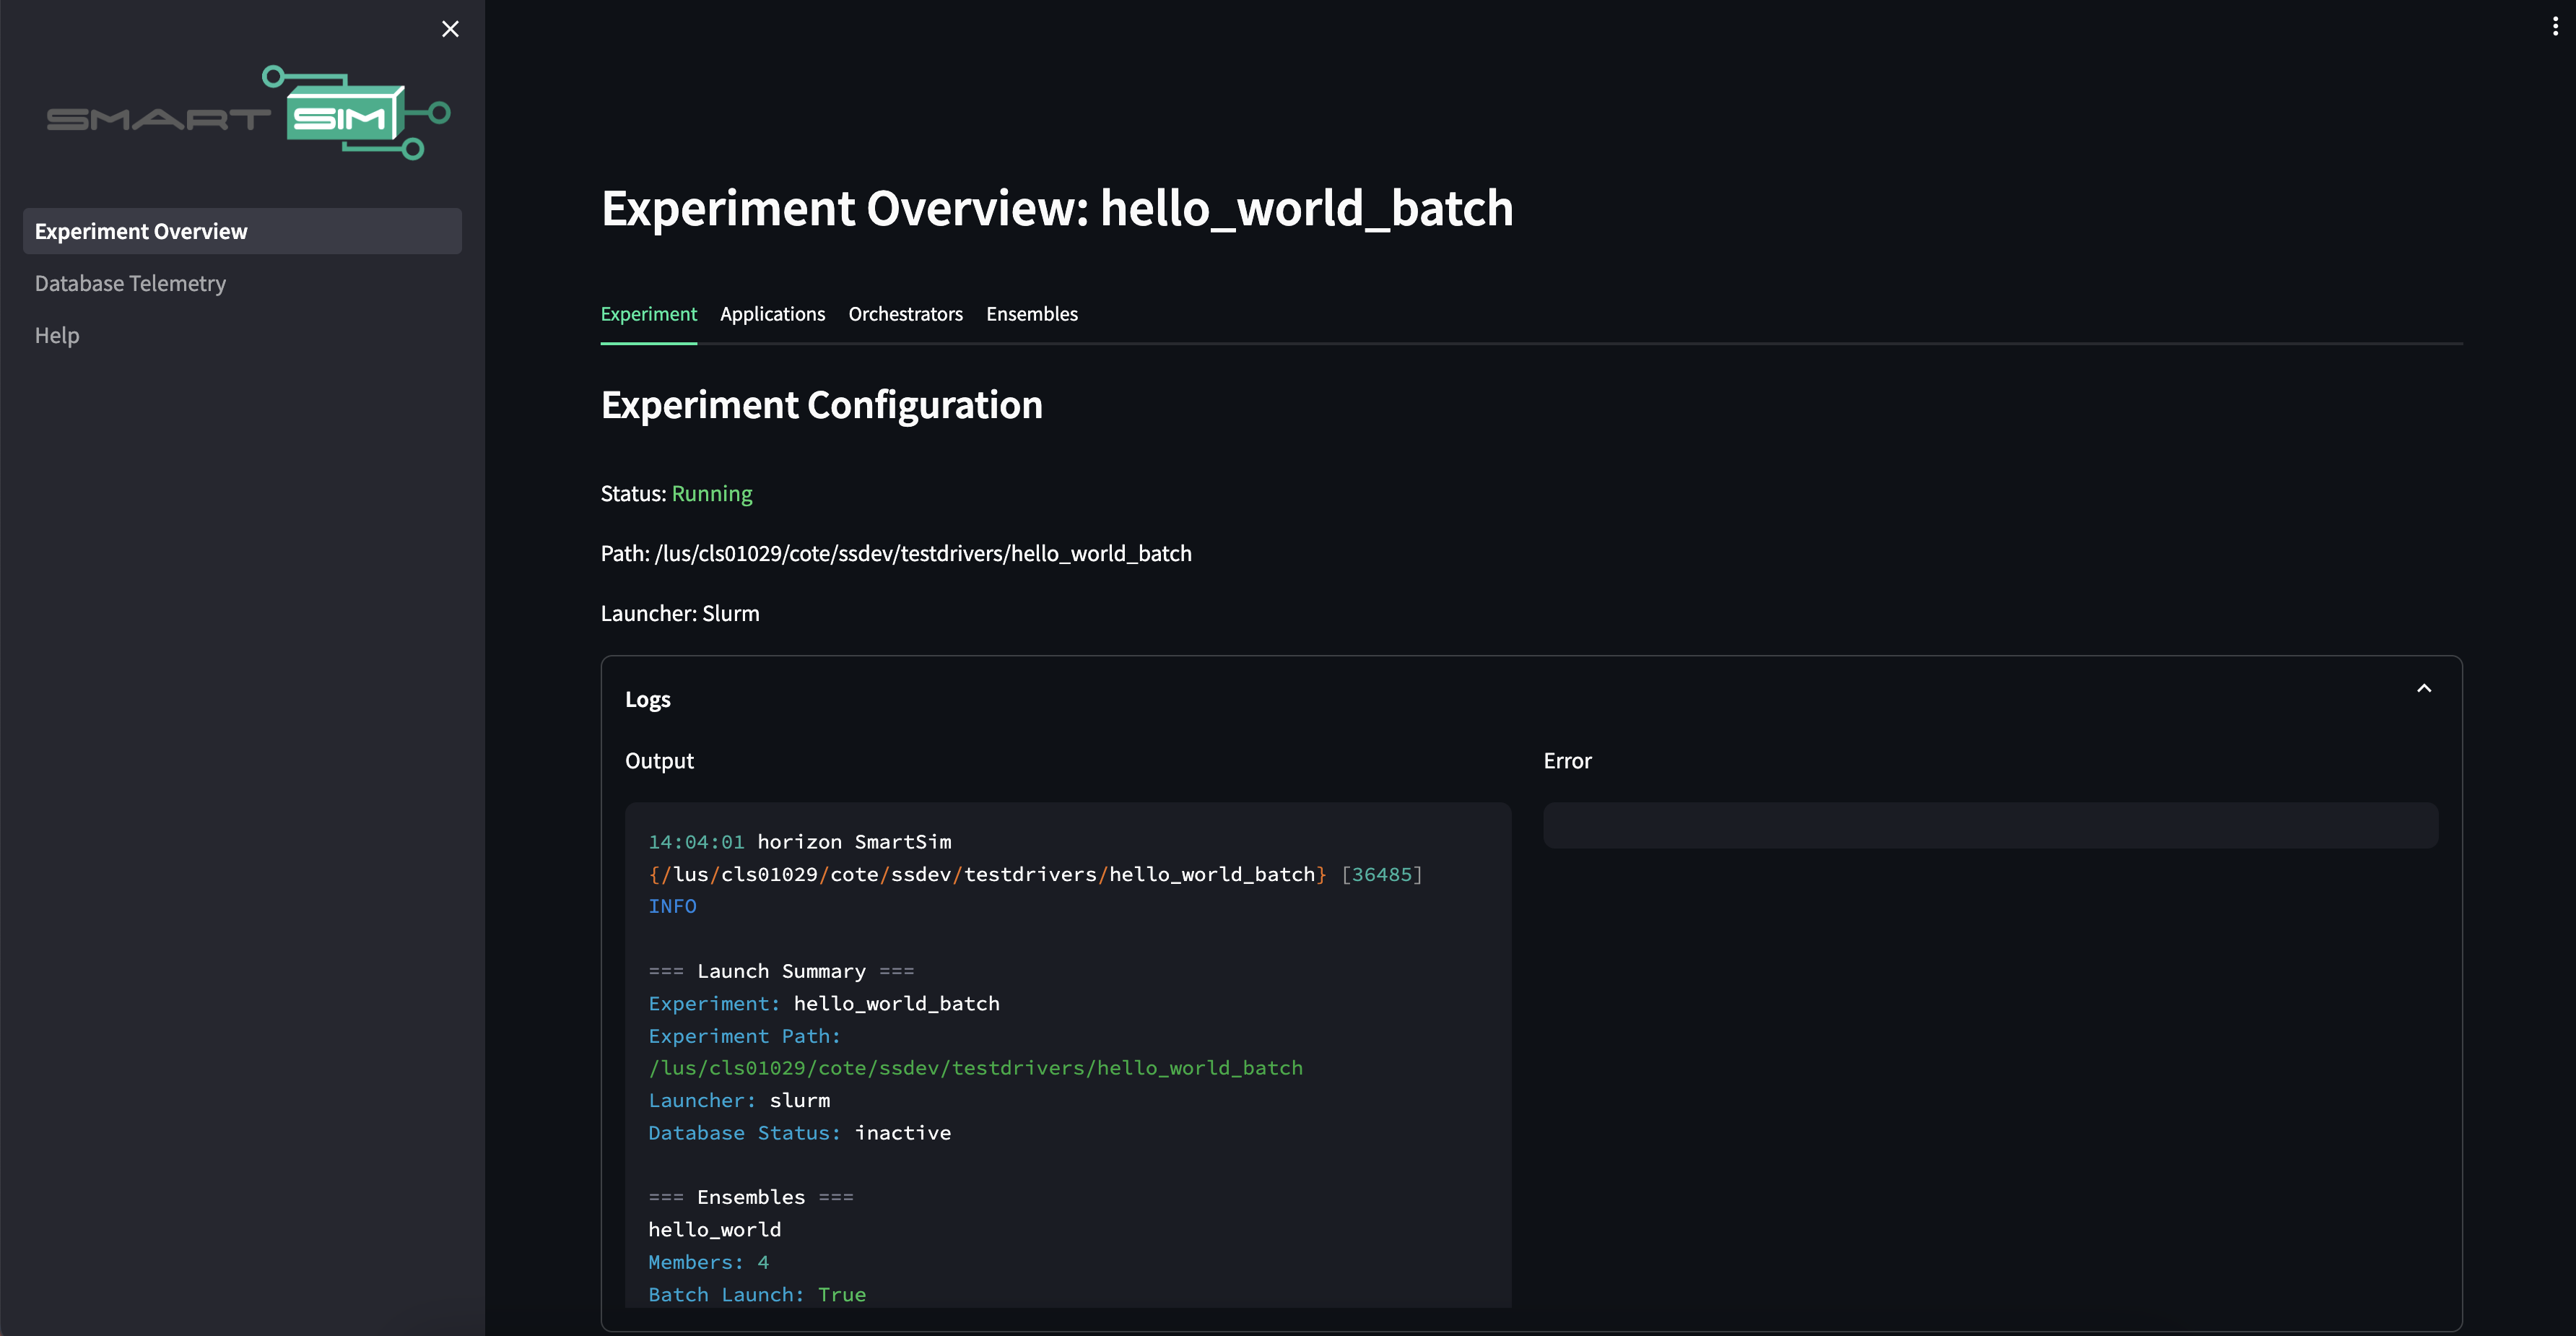
\includegraphics[width=0.8\columnwidth]{images/smartdashboard_experiment.png}
    \caption{The SmartSim Dashboard used by users to monitor the state of their experiment overall and individual components.}
    \label{fig:smartsim-dashboard}
\end{figure}

%%%%%%%%%%%%%%%%%%%%%%%%%%%%%%%%
\subsection{Cloudmesh}


Within HPC environments, scientific tasks can leverage the processing power of a supercomputer so they can run at previously unobtainable high speeds or utilize specialized hardware for acceleration that otherwise is not available to the user. HPC can be used for analytic programs that leverage machine learning applied to large data sets to, for example, predict future values or to model current states. For such high-complexity projects, there are often multiple complex programs that may be running repeatedly in either competition or cooperation, as also in the earthquake forecast application.  This may even include resources in the same or different data centers on which the benchmarks are run. 

To simplify the execution on such infrastructures, we developed a hybrid multi-cloud analytics service framework that was created to manage heterogeneous and remote workflows, queues, and jobs.  It can be used through a Python API, the command line, and a REST service. It is supported on multiple operating systems like macOS, Linux, and Windows 10 and 11.  The experiment workflow is specified via easy-to-define YAML files within cloudmesh.  

Cloudmesh was originally designed to provide an easy-to-use API, command line, and command shell to interface with various cloud and local providers. This includes managing compute resources on these providers, as well as accessing data stores. It is based on a Python API that allows the integration of functionality into other frameworks from the bottom up. 

In contrast to simple command line tools for cloud providers. cloudmesh provides not just command lines, but also a command shell at the same time. The command line execution is simply the execution of the command shell with a given set of inputs. Through this concept, you can create cloudmesh scripts that can be executed easily, in case you need a sequence of commands that need to be replicated.

Cloudmesh uses the Python package namespace feature to allow the definition of plugins to cloudmesh in different packages maintained in different files and directories. This is an important feature as it allows us to have contributions developed for cloudmesh by different developers.

At this time we support the namespace {\em cloudmesh} and any module developed can be installed into this namespace with a simple pip install. To simplify the development of new plugins, we provide a convenient plugin template generator that provides in source code a new command with all needed features such as setup, requirements file, and naturally a code template. 

The components of Cloudmesh that interface with cloud providers are based on the concept of abstract {\em providers} that make it possible to develop API interfaces for different services independently while inheriting the functionality from a common abstract class. To allow easy specification of such providers by the users, a YAML file is used to set them up. This allows the creation of predefined named instances on clouds by name. Similar features exist when working with file systems.
Furthermore, cloudmesh contains a prototype that can automatically generate REST services using OpenAPI specifications Python from functions and classes. 

More information about this part of cloudmesh is provided at \citep{www-cloudmesh-org}.

Next, we will focus on some of the newer components that explicitly deal with experiment workflows
and have been in part introduced in 
\citep{las-2022-hybrid} and
\citep{las-2022-templated}.


This includes a component called Experiment Executor (cloudmesh-ee) and Compute Coordinator (cloudmesh-cc). The first is responsible for executing experiments based on hyperparameters and system parameters, and the second allows such experiments to be integrated into a heterogeneous workflow that can be executed on multiple compute resources leveraging the appropriate scheduling system for that resource which is exposed through the Experiment Executor.

Hence, we provide the following functionality 

\begin{itemize}
\item {\bf (a) Heterogeneous System Integration:} the placement
of the workflow onto a number of different compute resources
including HPC, cloud, and local computing while also providing adaptations to various batch queues, 
\item {\bf  (b) Heterogeneous Compute Coordination:} the coordination of task-based parallelism to execute
the workflow on the various resources, and 
\item  {\bf (c) Heterogeneous Experiment
Execution:} the coordination of hyperparameter sweeps as well as infrastructure parameters used
in the application through the experiment coordinator.  

\end{itemize}

The architecture of the framework is depicted in Figures \ref{fig:cc-2} a and b. 

The framework is based on a layered architecture so that
it can be improved and expanded on at each layer targeting
developers and end users.

Obviously, the system can also be used on a uniform HPC infrastructure but the user can integrate into their workflow multiple systems at the same time if needed. This is the reason we use the term heterogeneous. Next, we describe the two components in more detail.

\begin{figure}[htb]

  \ifbool{SUBMISSION}{  
      \centering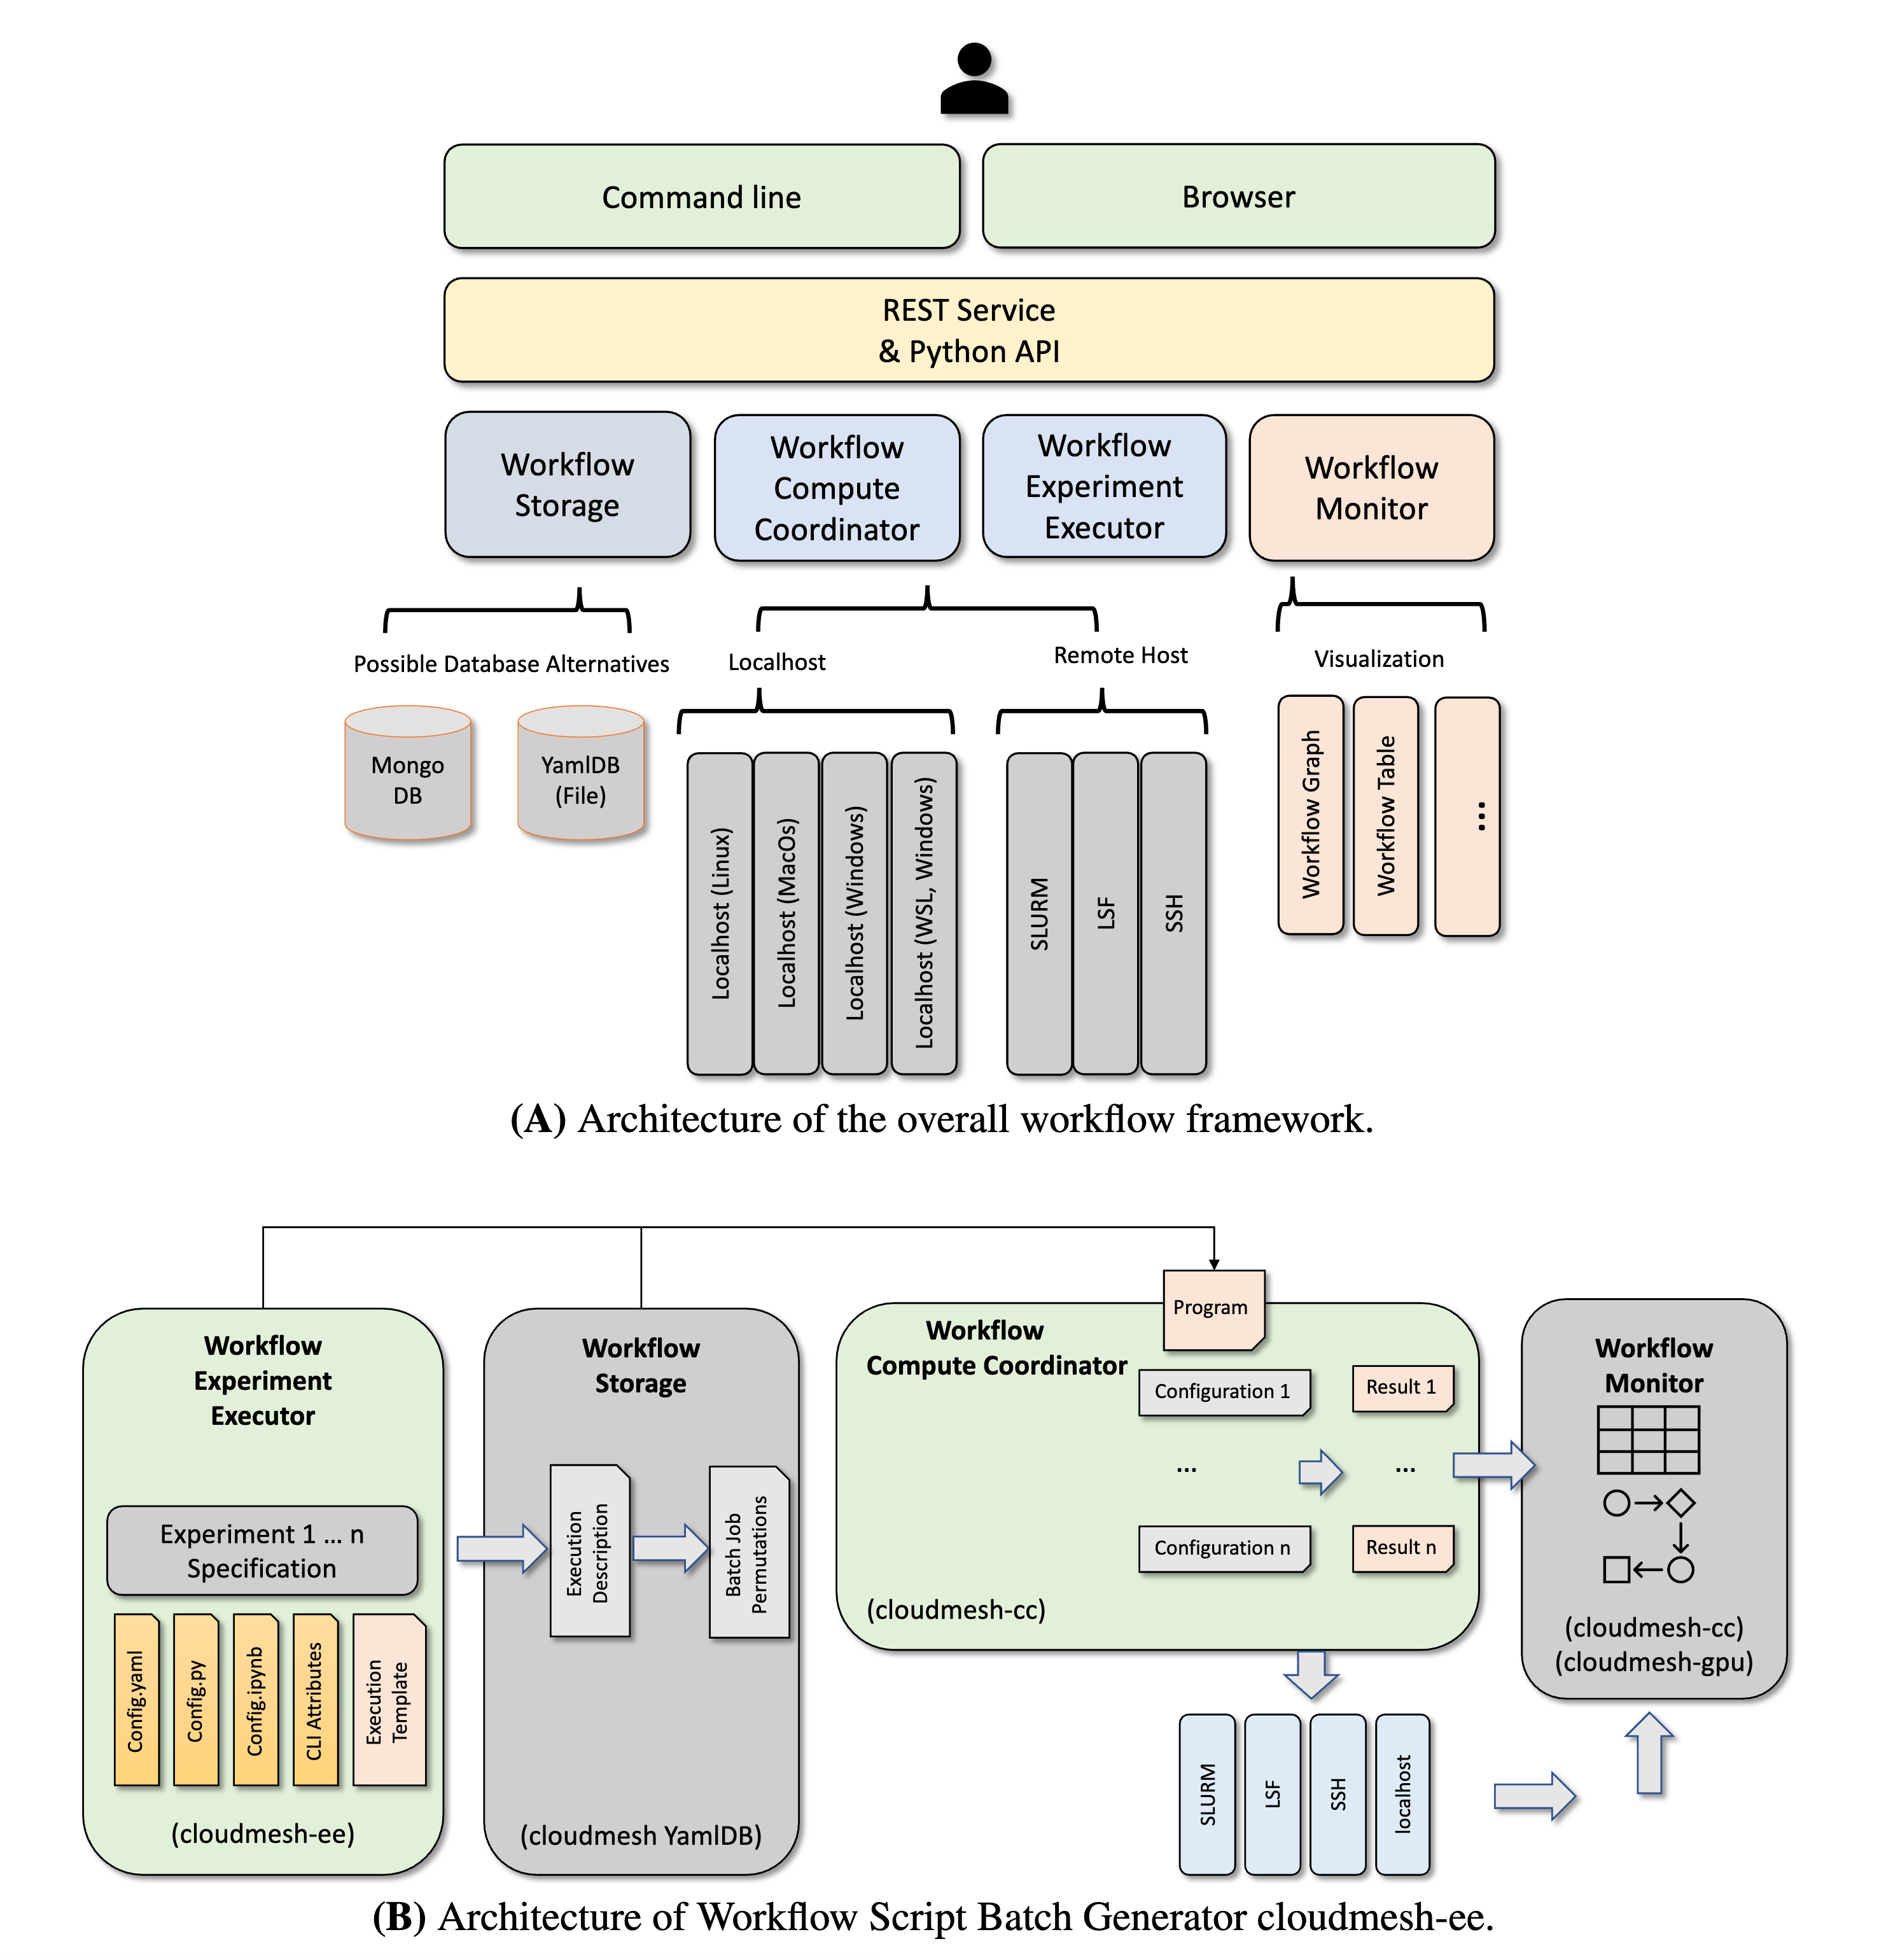
\includegraphics[width=1.0\columnwidth]{images/fig3}
  }{
    \centering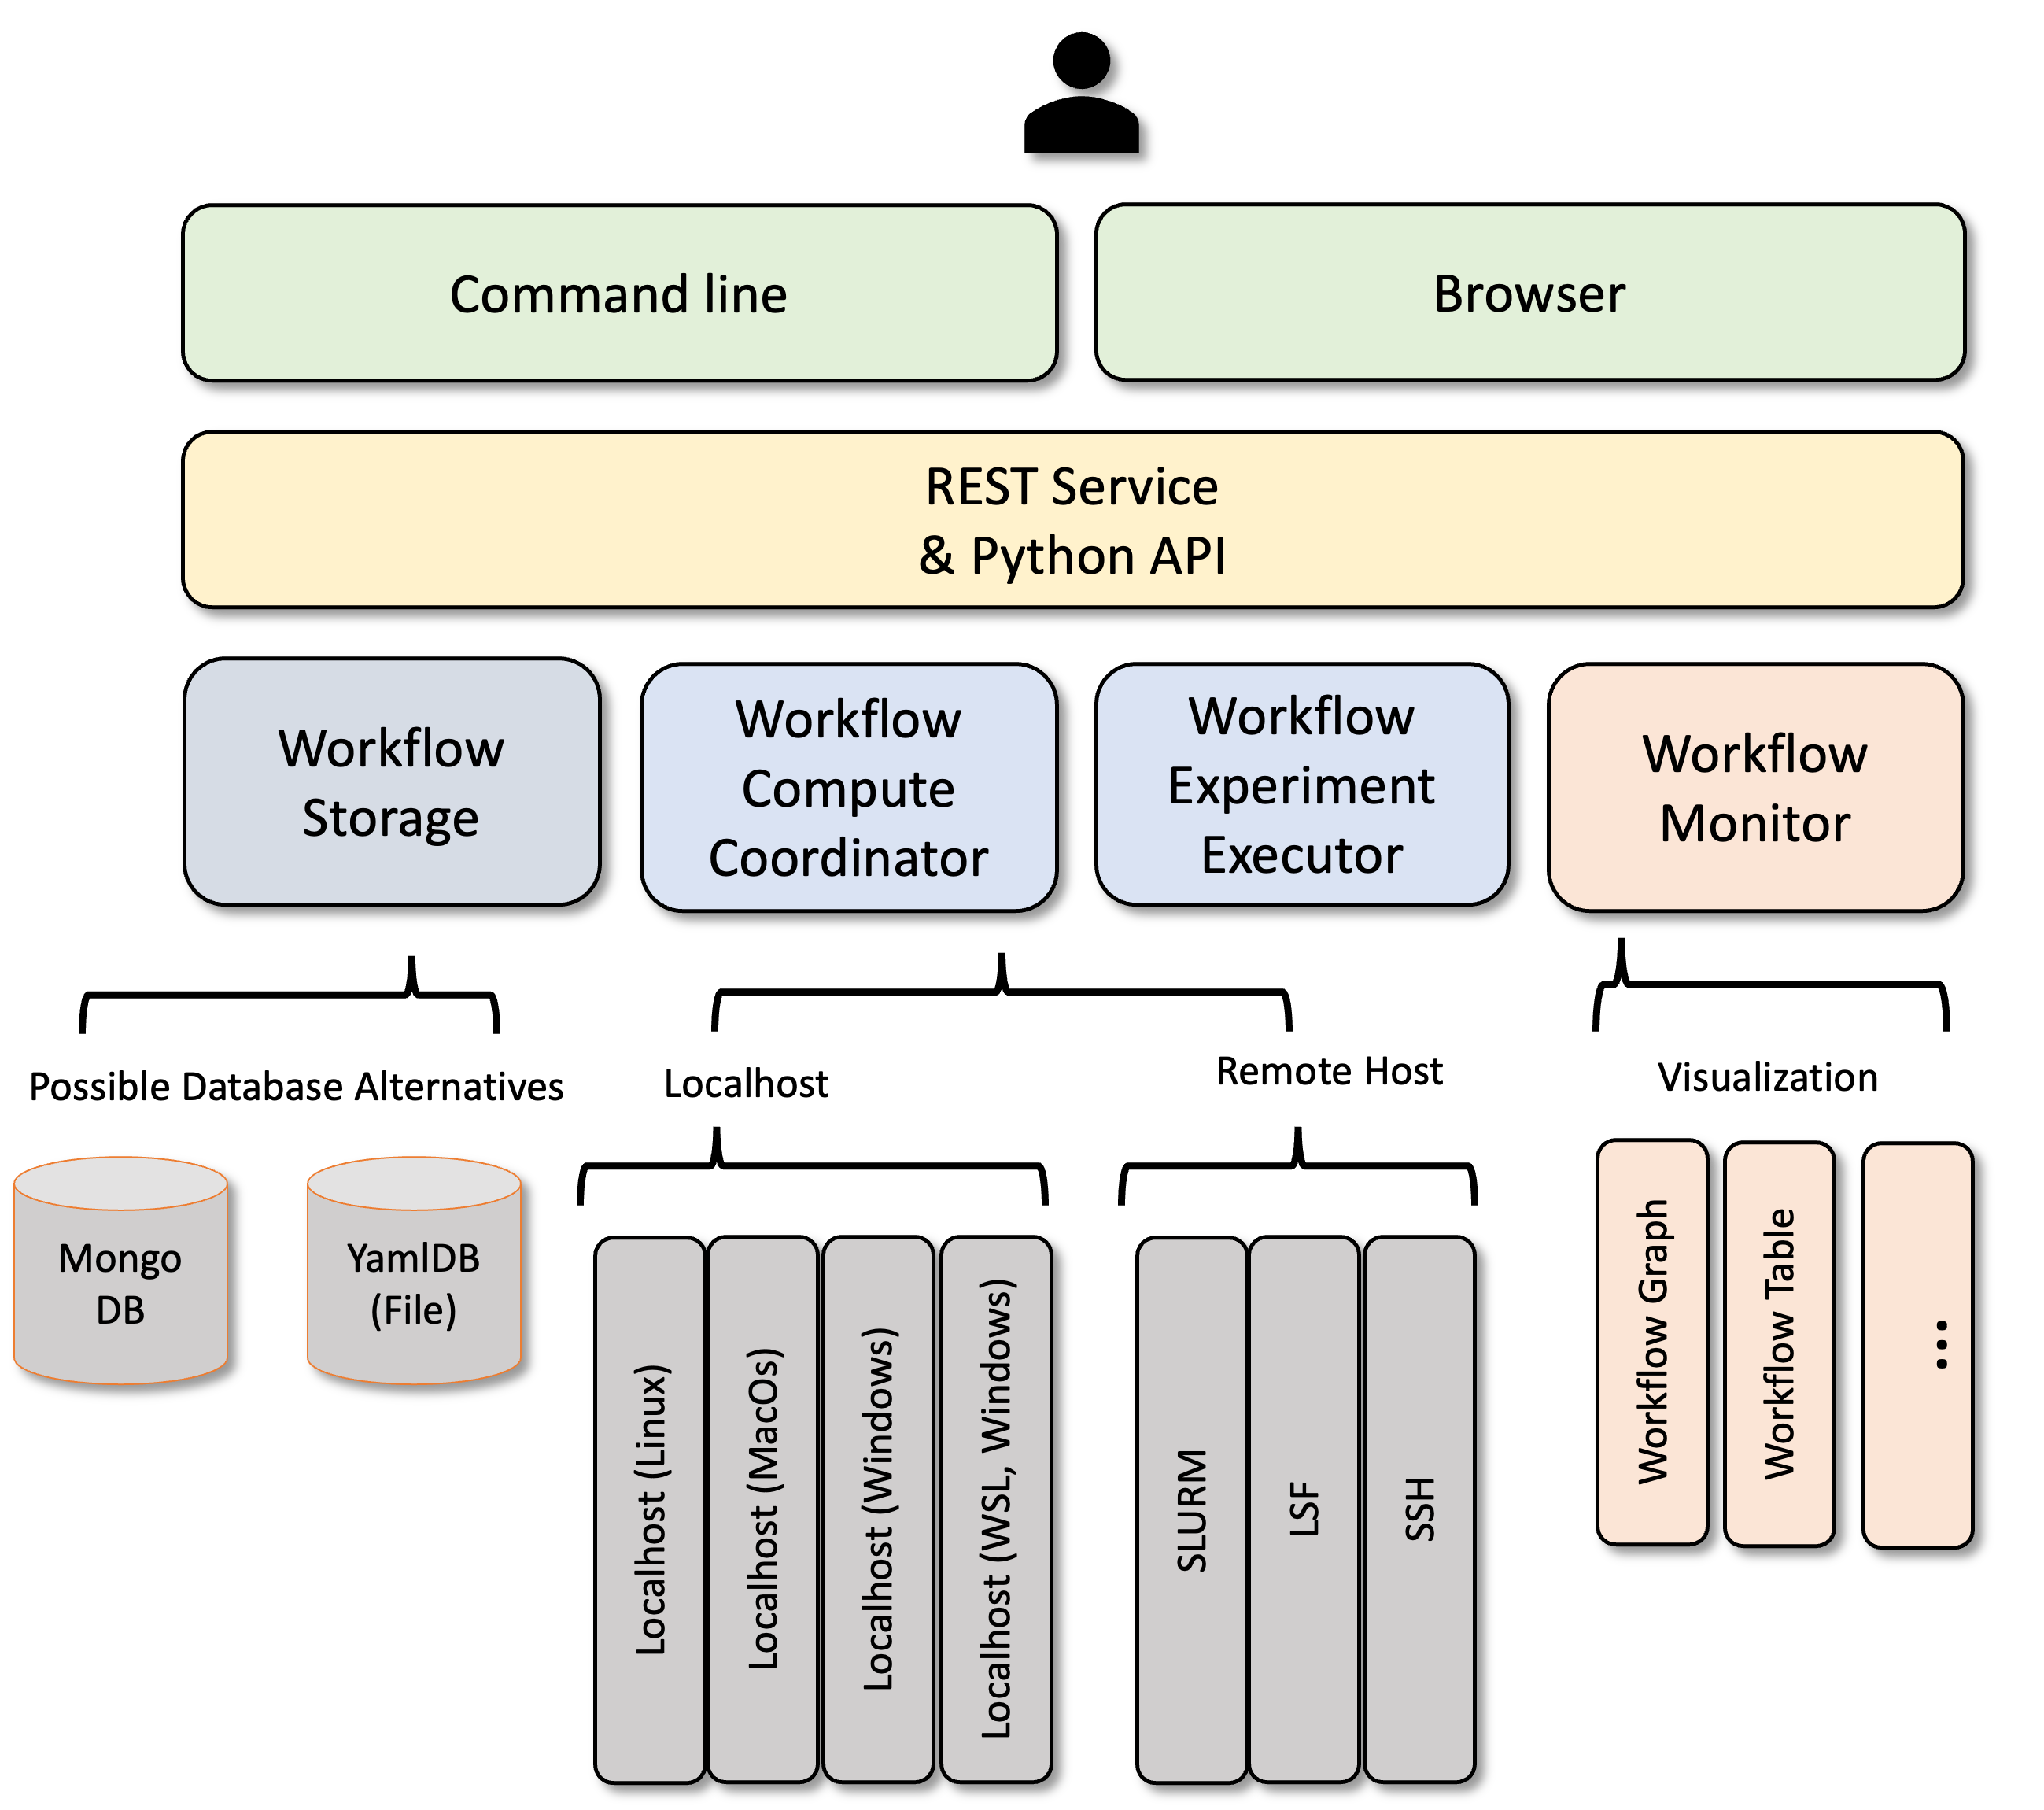
\includegraphics[width=0.70\columnwidth]{images/cloudmesh-cc-new}
    
    {\bf (A)} General architecture of the integrated Cloudmesh {\bf Compute Coordinator} and {\bf Experiment Executor} \citep{las-frontiers-edu}.

\bigskip\bigskip
    
    \centering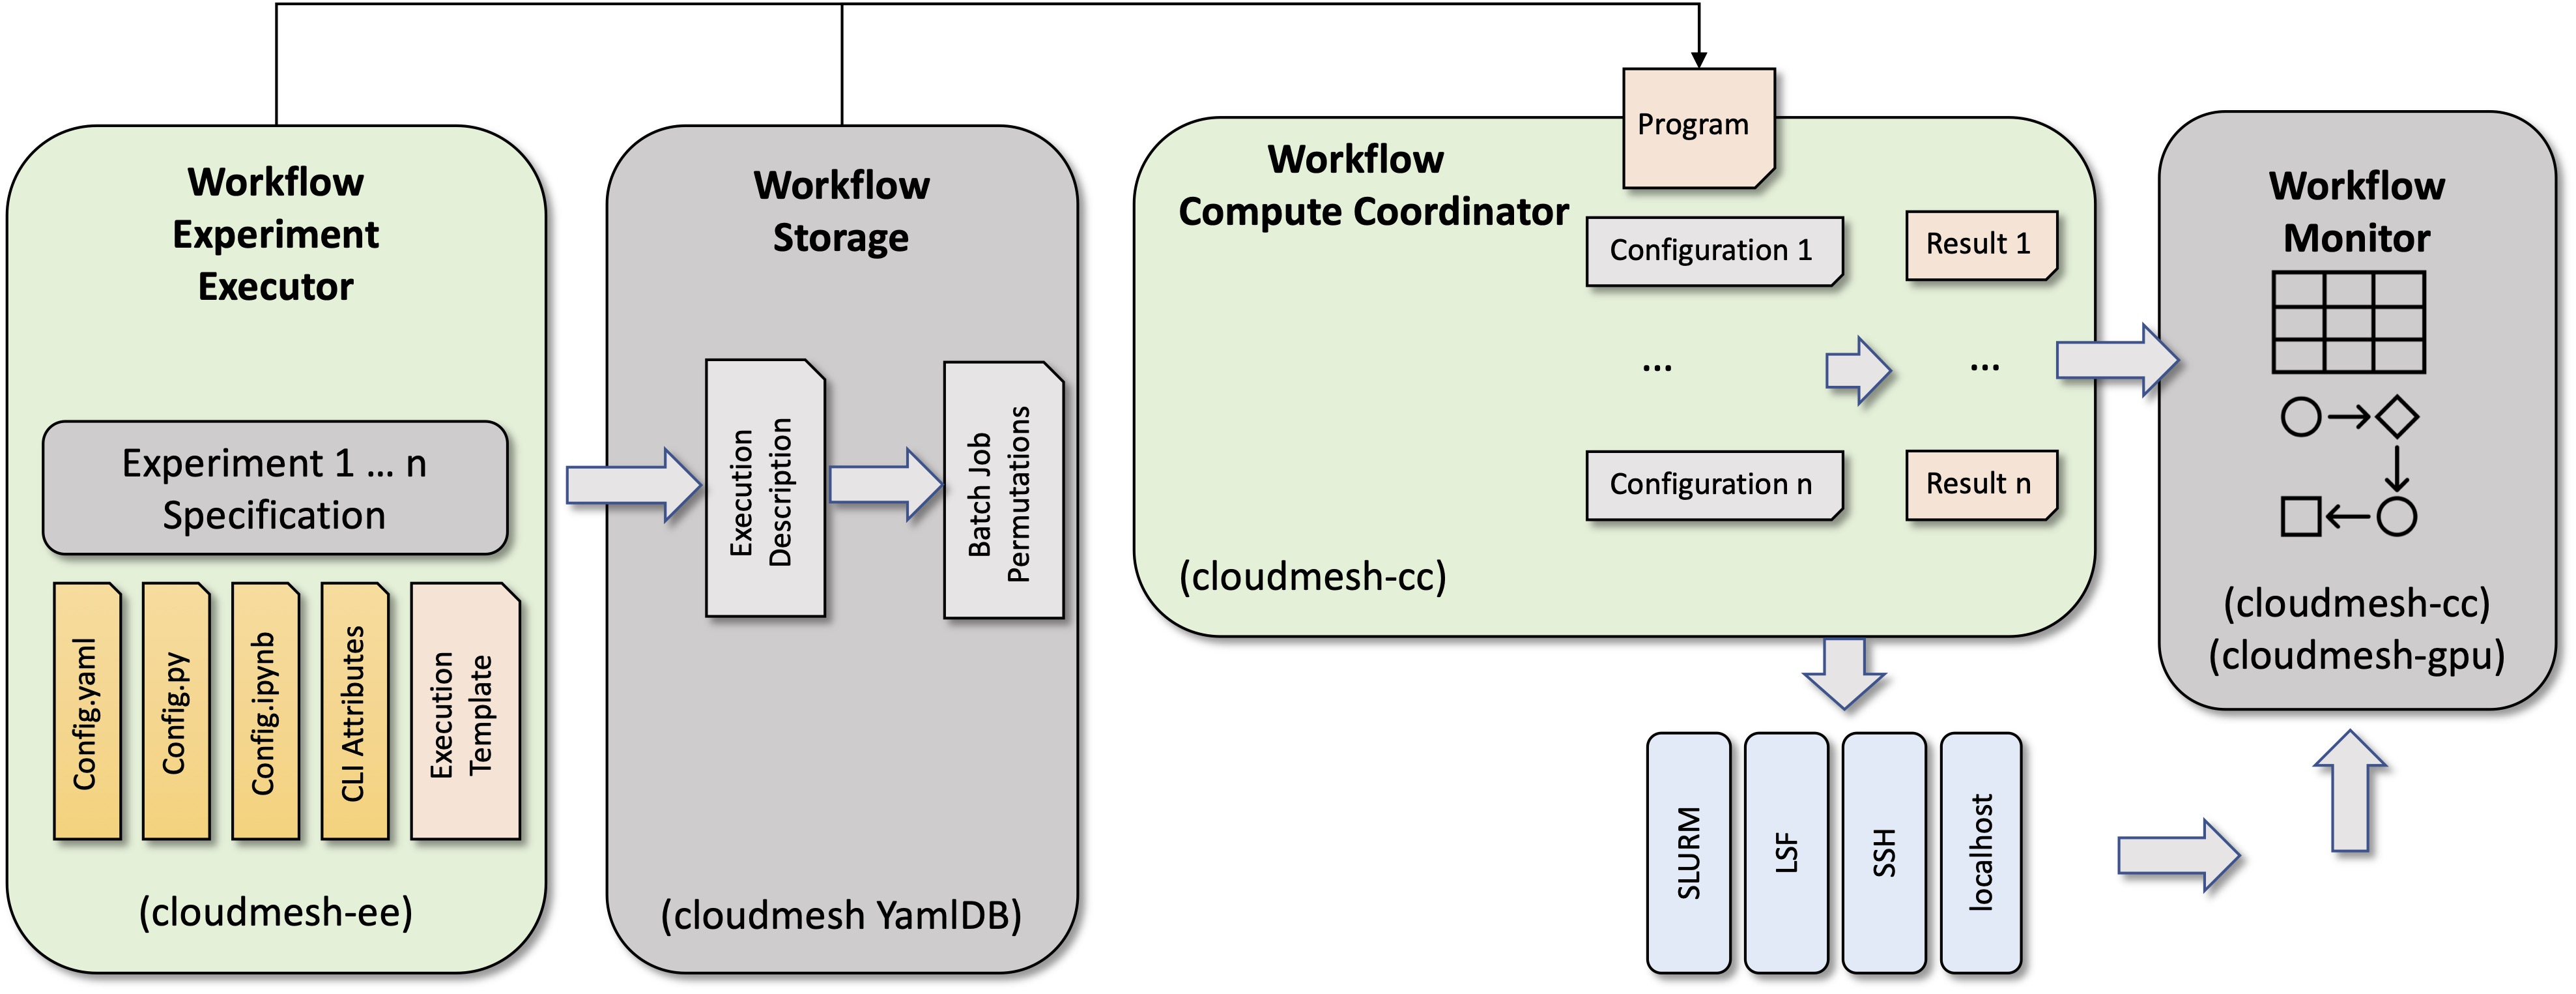
\includegraphics[width=1.0\columnwidth]{images/cloudmesh-ee-new}
    
    
    {\bf (B)} General architecture of Cloudmesh Experiment Executor interfacing with abstract schedulers \citep{las-frontiers-edu}.
  }

  
  
    \caption{Architecture of the Cloudmesh Workflow Service Framework.}
    \label{fig:cc-2}

\end{figure}


 
%%%%%%%%%%%%%%%%%%%%%%%%%%%%%%%%%%%%%%%%%%%%%%%%%%%%%%%%%%%%%%%%%%%%%%%%%%%%%%%%
\subsubsection{Compute Coordinator a Cloudmesh Plugin}
%%%%%%%%%%%%%%%%%%%%%%%%%%%%%%%%%%%%%%%%%%%%%%%%%%%%%%%%%%%%%%%%%%%%%%%%%%%%%%%
\label{sec:workflow-cc}

The role of the compute coordinator (CC) is to execute tasks on compute resources. Tasks can be scheduled on a variety of schedulers operating on compute resources. Examples are LSF, SLURm, and SSH.

The workflows are defined with human-readable YAML and can be stored in various formats on databases such as Cloudmesh file-based YamlDB \citep{yamldb}. Hence, it is easy to create a variety of add-ons to CC such as monitoring components that can be for example part of a Web browser-based implementation to display the Workflow and its status as a graph, table, or even as a continuous log file.  Tasks and Jobs report their status at runtime into the database.  To provide uniformity,  we have introduced an abstract job class that is integrated into a workflow class that allows us to define jobs, start them, and cancel them, to name only the most important management methods. Internally, each job creates a status file in which the actual progress of the job is recorded.  This status file is managed directly on the compute resource on which the job is run and is queried through pull requests on demand to return the status to the client. This way, the status of all jobs can be monitored easily. As we strive not to run jobs that execute not in milliseconds but rather in the multiple-second or hour range, such status reporting and propagation is well-suited for us because they are typically long-running.  As our status progress update specification is universally applicable via integration into notifications through files (including stdout and stderr) they can hence also be issued by bash scripts, SLURM scripts, Python programs, Jupyter notebooks, or any frameworks written in other computing languages. The workflow status updates are implicitly and uniformly augmented with timestamps, the compute resource, where it results from, and additional messages are appended to be sent to the monitoring component.  The workflow allows the specification of dependencies between tasks and supports a DAQ.
The code is compatible with Windows, macOS, and Linux.


The workflow specification plays an important role in not only defining a workflow but also in simplifying status updates that are updating an instantiation of a workflow. As we have completely separated the status of the workflow from obtaining status updates, the system allows it to be shut down while the underlying jobs as part of the system integration can still be executed and update their status managed on the remote resources. Once the system is started again on the user's local machine, it self-synchronizes its status from the system integration services that query the status of the appropriate resources. To summarize, the client is stateless and fetches the state of the submitted jobs on demand. It will return the latest state found on the job execution services.

The workflow definition for CC is rather simple and
intuitive and has been introduced in \cite{las-2022-templated} as the example in  Figure~\ref{fig:workflow-example} depicts. Here a graph
with the tasks ($start \rightarrow f\!etch\!-\!data
\rightarrow compute \rightarrow analyze \rightarrow end$) representing a typical minimalistic use case for Deep Learning (DL) is shown. The workflow
 executes three scripts ([fetch-data,compute,analyze].sh) while the dependencies are specified in a human-readable format using the names of the nodes. The nodes contain easy-to-manage information such as the name of the node, a label that is used to print the node's progress, and can contain templated variables such as any value defined as part of a particular node, or specially formatted time stamps. To demonstrate the easy use our label contains the {\em name} and {\em progress} of the workflow which is rendered by the graph or table monitoring components. One can also use variables accessible from Python including operating system or batch system variables to name only a few. Selected examples of values usable in the nodes are listed in \citep{las-2022-templated}.
As the format of the workflow is simple and easy to parse other interfaces can be created. We have provided in \ref{fig:gui-view} a view of a web browser-based interface that renders a workflow in either table or graph format. These are prototypes showcasing how easy it is to use existing tools to be utilized with CC to customize views. Another example is the ability to utilize OpenAPI as indicated in 
Figure \ref{fig:cc-3}  which allows the access of the functionality as part of a REST service with appropriate specification. 

%It is interesting to note that the same concepts of specifying a workflow in a scripted fashion have been used in our earliest work \cite{las-94-ecwmf}. However, at that time YAML was not yet invented and we used our own specification language.  

\begin{figure}[htb]
\vspace{-0.4cm} 
\begin{lstlisting}[breaklines=true]
(*\bfseries workflow:*)
  (*\bfseries nodes:*)
    start:
       name: start
    fetch-data:
       name: fetch-data
       user: gregor
       host: localhost
       status: ready
       label: '{name}\nprogress={progress}'
       script: fetch-data.sh
    compute:
       name: compute
       user: gregor
       host: localhost
       status: ready
       label: '{name}\nprogress={progress}'
       script: compute.sh
    analyze:
      name: analyze
      user: gregor
      host: localhost
      status: ready
      label: '{name}\nprogress={progress}'
      script: analyze.sh
    end:
       name: end
  (*\bfseries dependencies:*)
    - start,fetch-data,compute,analyze,end
\end{lstlisting}
\vspace{-0.4cm}
\caption{Workflow YAML Configuration file.}\label{fig:workflow-example}
\label{fig:yaml-file}
\end{figure}




\begin{figure*}[htb]
\begin{minipage}[t]{0.49\columnwidth}
\centering  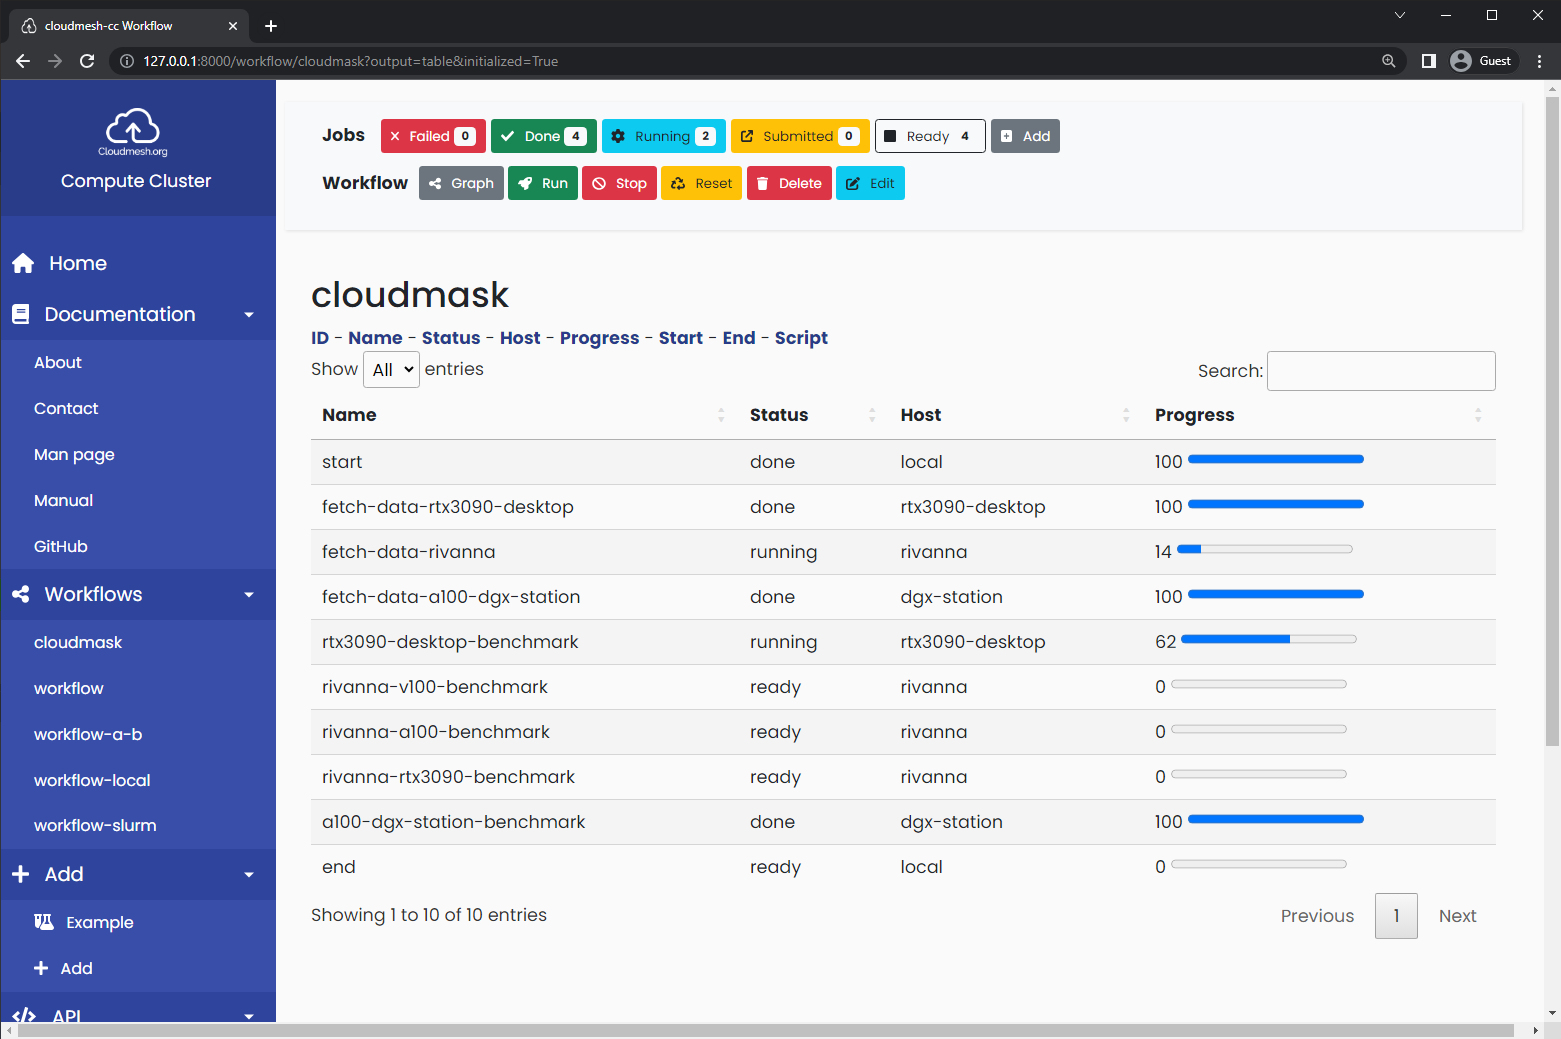
\includegraphics[width=1.0\columnwidth]{images/table-cloudmask-workflow.png}
%\caption{Table view.}
%\label{fig:table-view}
\end{minipage}
\hfill
\begin{minipage}[t]{0.49\columnwidth}
  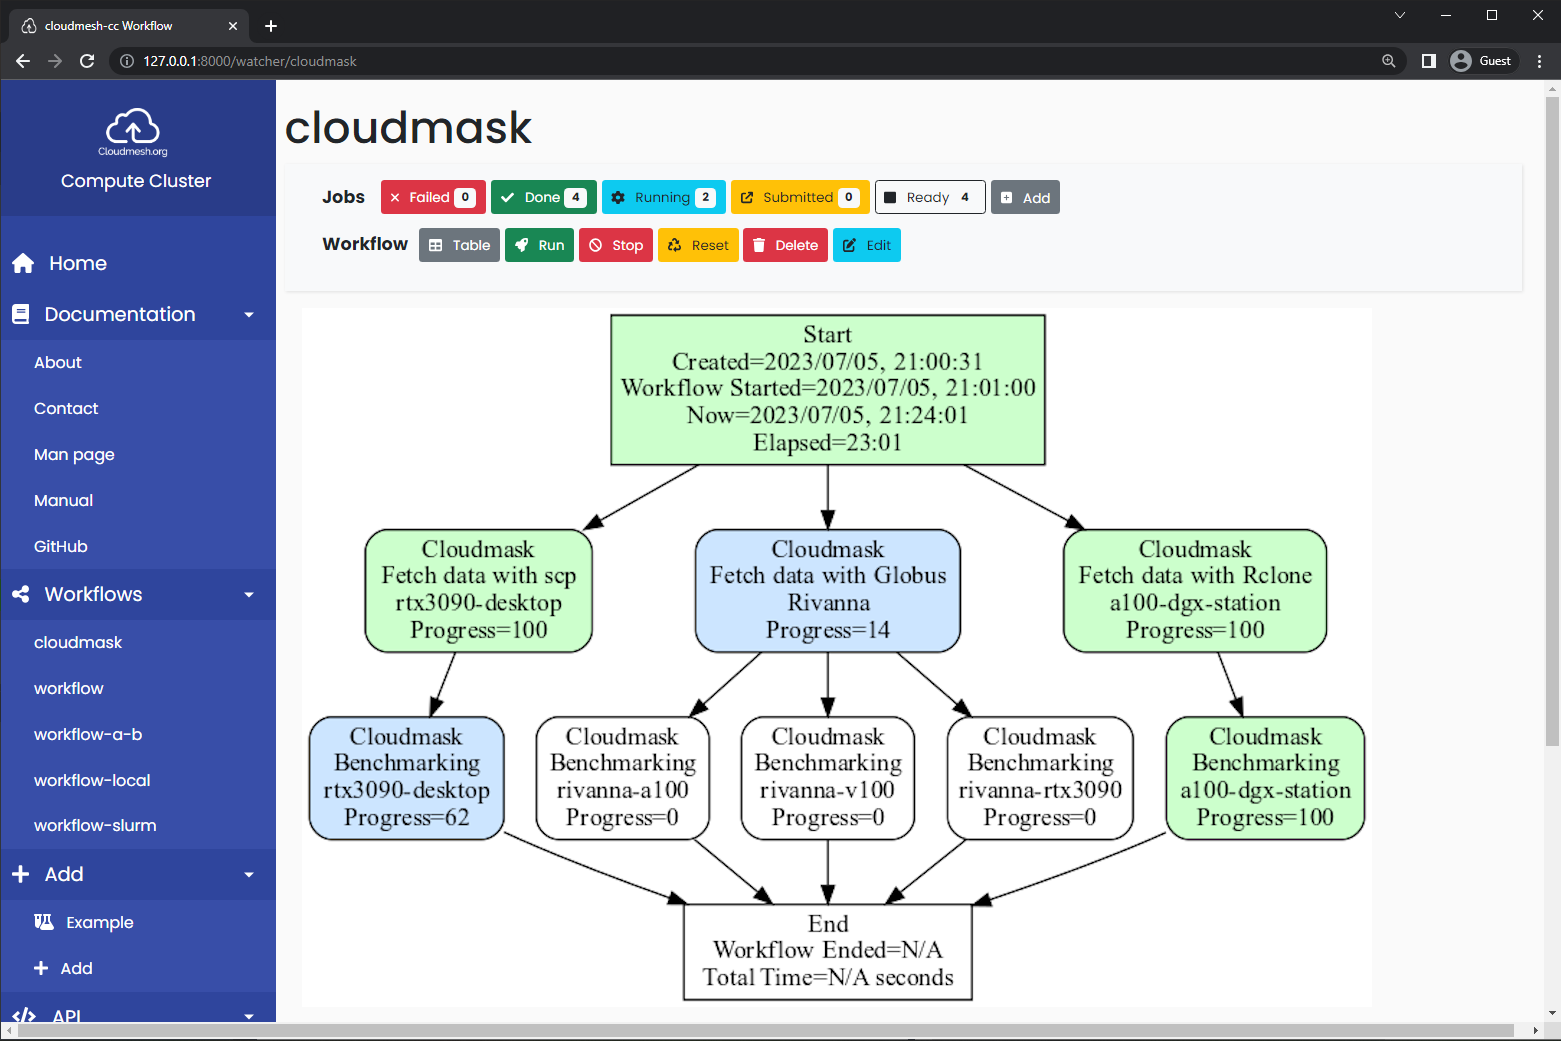
\includegraphics[width=1.0\columnwidth]{images/gui-cloudmask-workflow.png}
\end{minipage}
 \caption{Table and Graph view of CC workflow}
\label{fig:gui-view}
\vspace{-0.5cm}
\end{figure*}


\begin{figure}[htb]
    \centering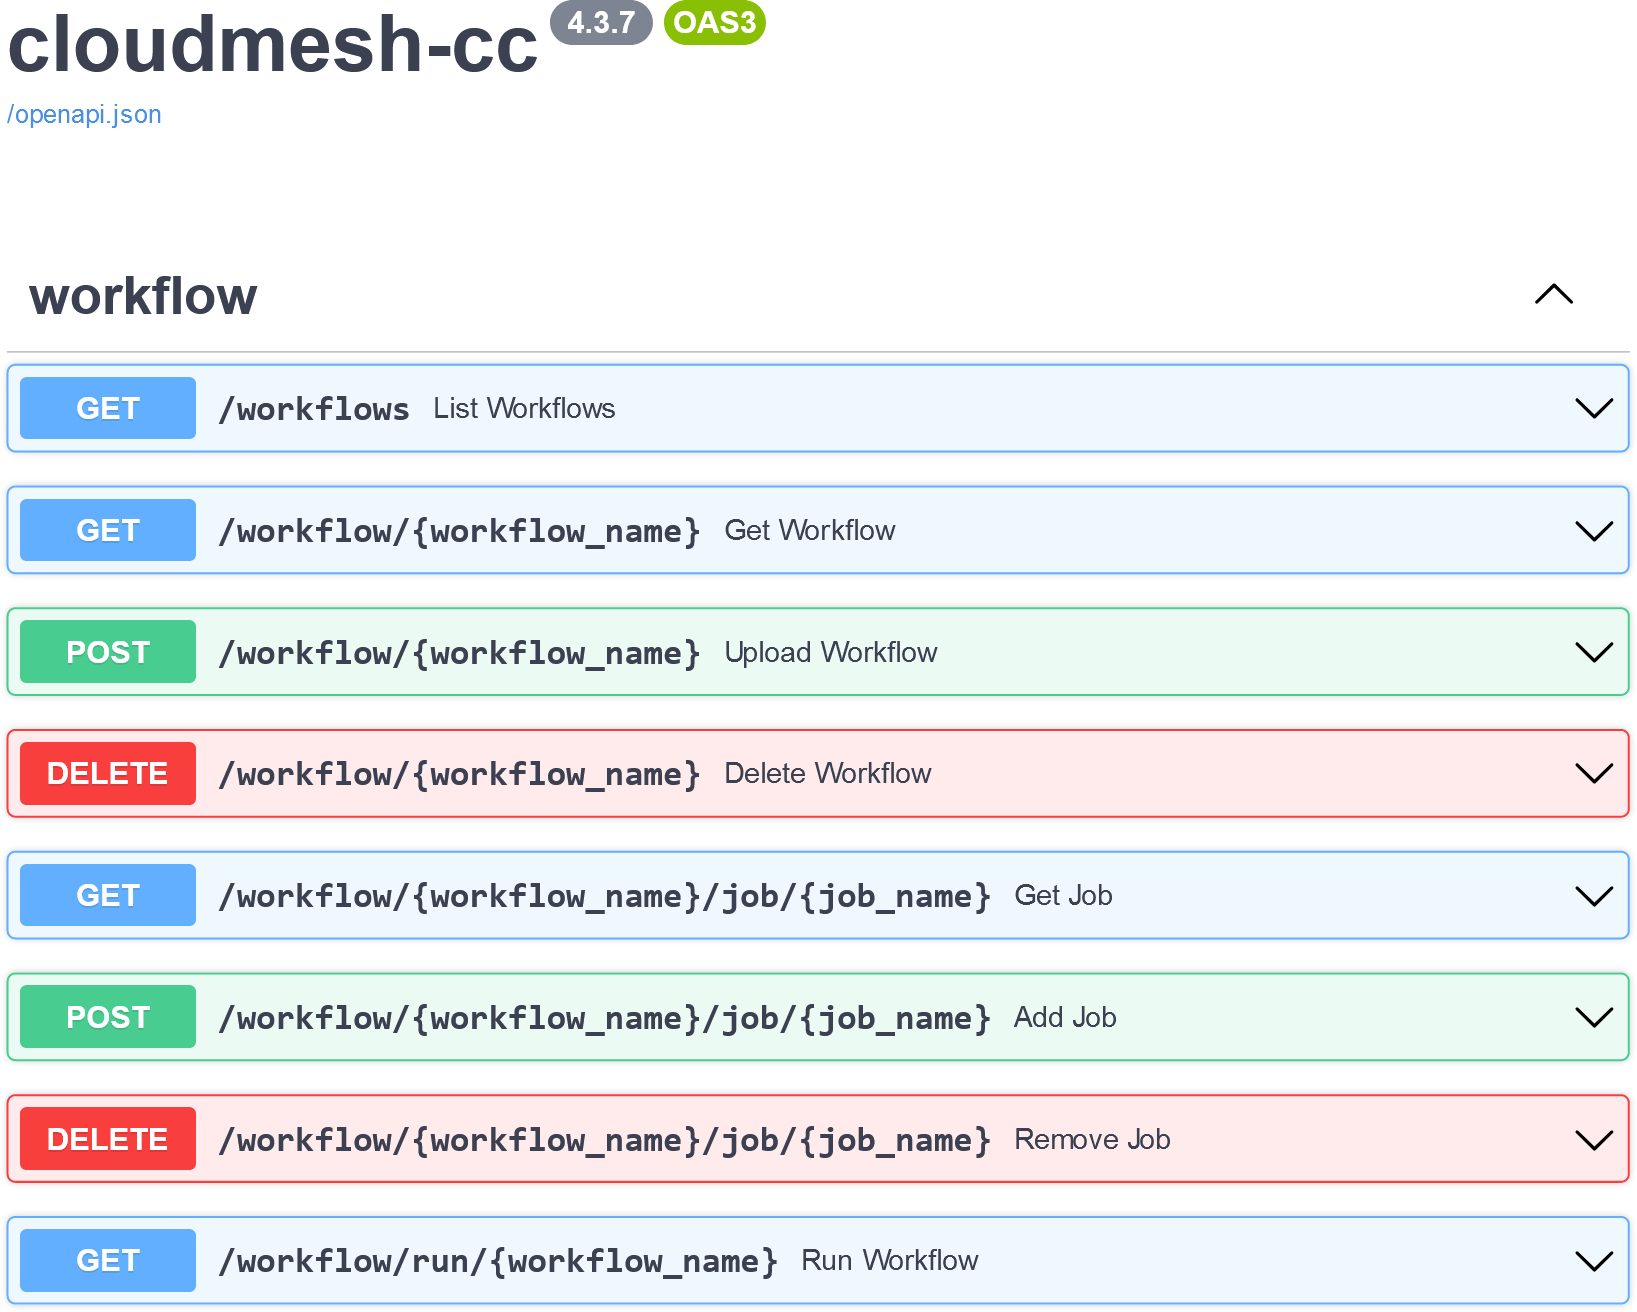
\includegraphics[width=0.49\columnwidth]{images/fastapi-service-highres.jpg}
      
    \caption{OpenAPI workflow service Workflow interfaces.}
    \label{fig:cc-3}
\end{figure}





%%%%%%%%%%%%%%%%%%%%%%%%%%%%%%%%%%%%%%%%%%%%%%%%%%%%%%%%%%%%%%%%%%%%%%%%%%%%%%%%
\subsubsection{Experiment Executor a Cloudmesh Plugin}
%%%%%%%%%%%%%%%%%%%%%%%%%%%%%%%%%%%%%%%%%%%%%%%%%%%%%%%%%%%%%%%%%%%%%%%%%%%%%%%

\label{sec:workflow-ee}

The Experiment Executor (EE) \citep{las-frontiers-edu} allows the execution experiments defined by experiment parameters to be used at runtime for the execution of multiple experiments. It is motivated by two kinds of parameters. 
In traditional machine learning workflows and benchmarks, hyperparameter tuning and configuration are key elements in assessing and optimizing the performance of models. However, scaling hyperparameters for highly parallel execution with heterogeneous hardware is complex. EE is used to generate many parameter combinations in a Gridsearch. Besides hyperparameters, EE also allows the specification of resource-specific parameters determining hardware and even software properties when an experiment is executed.

The architecture of the cloudmesh-ee framework is depicted in Figure \ref{fig:cc-2}B.

EE experiments can utilize various queuing systems such as SLURM, and LSF, but also sequential and parallel ssh jobs. The scheduling of the jobs to be executed could be customized. Besides static gridsearches, EE can also leverage functions and introduce runtime dynamically changing searches.

As a result, the output structure of the experiment includes the hyperparameter values, providing a unique identifier for each experiment, the results from different computing systems can be merged into the overall combined results. Thus the EE supports the creation of coordinated results while allowing the generation of cooperating, selective, and distributed result generation. A simple experiment configuration file is shown next, where we execute a scientific application called cloudmask for epochs 1, 30, and 60, on the GPUs v100 and a100 repeating it 5 times.

{\scriptsize
\begin{lstlisting}[breaklines=true]
    application:
        name: cloudmask
    data: "/scratch/{os.USER}/{application.name}"
    experiment:
        epoch: "1,30,60"
        gpu: "a100,v100"
        repeat: "1,2,3,4,5"
\end{lstlisting}
}

Dependent on the queuing system a custom templated batch script is created by EE so it can be easily executed when desired.
As the templated experiments are user-independent, it can then also be executed via different user accounts and even organizations if desired. Through the integration with cloudmessh EE can also use an energy monitor to create energy traces at runtime. This can be especially important for those also considering energy-related benchmark comparisons. As the overall experiment can be designed in chunks it is possible to create first experiments with a smaller runtime in order to estimate the impact larger experiments have on the runtime. 

While practically working with the system, we observed that students (as part of research experiences) not using our experiment executor spend a significant amount (weeks-months) of a semester on setting up a benchmark and replicating only a fraction of the functionality provided by the EE. However, we tested the system out while other students used EE and we observed that the applications for which a template and configuration file has been designed reduced the on-ramp time to less than a day. Not only that, instead of needing a team including graduate students, the work could be performed by a single undergraduate student student.

We have tested CC while running various applications including MNIST, Multilayer Perceptron, LSTM (Long short-term memory), Auto-Encoder, Convolutional, and Recurrent Neural Networks, Distributed Training, and PyTorch training.  A much larger application using earthquake prediction has also been used. Results of using it outside of the earthquake code are available in 
\cite{las-2023-escience}.

Cloudmesh-ee differentiates itself from other approaches as gridsearches can trivially be formulated either as API calls or as displayed here through an easy-to-understand YAML file. Through this mechanism, thousands of independent experiments can be run as part of a large-scale experiment workflow.

Cloudmesh-ee takes two configuration files. The first is a YAML file that includes all parameters used by the benchmark including an experiment section that defines the Cartesian product (or dynamic changing values in case a function is defined and used). The second is a SLURM template. From these files, it will create, for example, SLURM scripts via the {\em cms ee} command line and shell tool while

\begin{enumerate}
  \item using a unique directory for the experiment
  \item taking a parameter set from the Cartesian product of the experiment parameters
  \item creating from a batch job template an instantiation of the template while replacing all variables from the configuration file    and replacing the specific experiment parameters
  \item creating an instantiation of the configuration file while replacing all experiment parameters with the one for the current experiment.
\end{enumerate}

An example of a configuration file \verb|config.yaml| where we iterate over epochs, GPUs, and repeat it 5 times is shown next:

\begin{lstlisting}[language=sh]
    #!/bin/bash

    #SBATCH --job-name={experiment.repeat}-{application.name}
    #SBATCH --nodes=1
    #SBATCH --gres=gpu:{experiment.gpu}:1
    #SBATCH --time=02:00:00
    #SBATCH --mem=64G
    #SBATCH -o {experiment.gpu}-{application.name/{experiment.repeat}-%j.out
    #SBATCH -o {experiment.gpu}-{application.name}/{experiment.repeat}-%j.err
    #SBATCH --partition=bii-gpu
    #SBATCH --account=bii_dsc_community

    export USER_SCRATCH=/scratch/$USER
    cd USER_SCRATCH
    mkdir -p $USER_SCRATCH/{experiment.gpu}-{application.name}/%j.out
    (*\textcolor{blue}{nvidia-smi}*)

    cms gpu watch --gpu=0 --delay=0.5 --dense > outputs/gpu0.log &

    python earthquake.py --config config.yaml

    seff $SLURM_JOB_D
\end{lstlisting}
%$

Variables can easily be referred to with a dot notation in the templates.  Variables in the YAML file can also be replaced so it is possible to use abbreviations in a consistent fashion within the YAML file as well as in the batch script.

The configuration files can also determine the creation of output directories and files while assuring to place them in a predetermined unique but unifying order.

An example of a variable replacement specification in the YAML file is given for the \verb|data| value where not only the operating system variable \verb|os.USER| is replaced, but also the variable \verb|{application.name}|. Obviously, this is a significant functionality enhancement to a typical YAML file while still keeping it readable.  Multiple values for a variable are possible under the experiment tag, where a variable with multiple values is assigned a string of comma-separated values. 

Users now can use common variables value expansion to create experiments. Examples include graphics processing units, memory, file systems used, versions of Python, versions of TensorFlow, epochs, learning rate, and many other important parameters that can influence the benchmark.  

The intermediate output of EE ``is a shell script that contains all jobs that are to be executed with the defined permutations over the parameters. One nice side effect of this is that the jobs in the file can be run in parallel and have the queuing system take over the scheduling of the job following the system-defined queuing policies. However, it may also be possible to create a {\it collaborative group} submission, using our earlier introduced collaborative pattern, where multiple users submit a portion of the jobs so that policies restricting the number of jobs per user can be avoided. Furthermore, if access to multiple HPC machines is available the jobs could be split among the different machines. However, in that case, time measurements may not be a useful parameter to benchmark. However, as in the science group, we are concerned about accuracy the combination of a system comprised of multiple resources is meaningful \citep{las-2022-templated}.''


\subsubsection{Cloudmesh Benchmark Plugings}
\label{sec:monitoring}

We have observed that many of our students spend too much time augmenting their code with timers in an uncoordinated fashion. Therefore, we have provided a simple Python library that can be installed with pip so students can augment their codes in a most simple fashion. The important part is that EE and CC also use their library and thus an experiment has a consistent reporting function throughout.  Furthermore, we have made an extension so that it also directly returns in addition to the cloudmesh timer format, timers used by MLCommons in mllog format. The advantage is that the timers in cloudmeh format are humanly readable, while when also exporting mllog such benchmarks fulfill the MLCommons logging conventions. Besides these formats, the StopWatch also produces summary tables in txt, csv, HTML, JSON, and YAML. Furthermore, ti includes the automatically detected specification of operating systems parameters, which comes in handy when an experiment is to be replicated or further analyzed.
We show next  a use case that demonstrates how easy it is to use the StopWatch


\begin{lstlisting}[language=Python]
    from cloudmesh.common.StopWatch import StopWatch 
    # ...
    StopWatch.event("start")       # this where the timer starts
    StopWatch.start("earthquake")  # this is when the main benchmark starts
    # ... run the earthquake code
    # ... additional timers could be used here
    with StopWatchBlock("calc"):   # this is how to use a block timer
       run_long_calculation()
    StopWatch.stop("earthquake")   # this is where the main benchmark ends
    StopWatch.benchmark()          # prints the current results
\end{lstlisting}

To also have direct access to MLCommons events, we have recently added the ability to call a StopWatch.event.

In addition, we developed a simple command line tool to augment batch scripts to monitor the GPU performance characteristics such as energy, temperature, and other parameters \citep{cloudmesh-gpu}. It  can be started in a batch script and is currently supporting NVIDIA GPUs:


\begin{lstlisting}[language=sh]
    cms gpu watch --gpu=0 --delay=0.5 --dense > gpu0.log &
\end{lstlisting}


Monitoring time and system GPU information can provide significant insights into the application's performance characteristics. Hence, it is significant for planning a time-effective schedule for parameters while running a subset of planned experiments.


\subsection{Using Cloud Clusters in Cloudmesh Plugin}
\label{sec:cloudcluster}

Although our paper does not address cloud-provisioned resources much, we report here on a new development we started over the last several months. It describes our high-level API and abstractions to provision an HPC cluster in the cloud while the implementation concretely on AWS services. Nevertheless, it could be enhanced to other cloud providers offering similar services.

AWS Parallel Computing service (PCS) simplifies the infrastructure deployment of High Performance Computing (HPC) clusters on Amazon Web service cloud infrastructure. \citep{awspcs}. It creates an abstraction layer for the end user such as scientists who intend to run their experiments on such resources in a cloud eliminating costs to deploy and manage an HPC center. As the researchers are obviously not in the business of provisioning such resources, and may also not be familiar with the terminology and practices used in AWS to do it, they need to have a much simpler entry point in using AWS parallel clusters.
This way they can focus on the outcomes of the experiments rather than spending time in building the infrastructure required to run their experiments. The cloudmesh create plugin provides necessary automation that enables users to deploy clusters within minutes. Using cloudmesh create a fully functional HPC cluster  (AWS uses the term parallel cluster or PCS) can be built in about 6 minutes. 

The cloudmesh create plugin not only automates the cluster creation process, it goes much beyond that. It creates a head node, a worker node-group with a minimum capacity of 0, and a queue. The worker node minimum capacity of 0 is intentional in order to keep cloud costs in control. Users can login to the head node to interact with the cluster, and submit Simple Linux Utility for Resource Management (SLURM) jobs. This provides users with a seamless experience that they are used to work with on-premise HPC clusters. The nodes of the HPC can utilize a variety of compute options, starting from low-cost options for basic compute performance to the highest level of performance provided by Graphical Processing Unit (GPU) based instances. Multiple node groups can be created, and each node group can use the same or a different instance type. This flexibility allows for running different types of workloads on the same cluster. These node groups can be deleted when not in use to keep cloud costs in control. The auto-scaling feature of node groups allows users to define a minimum and maximum number of nodes, depending on the workload demand nodes within the node groups are automatically added and removed.


PCS supports a variety of shared file systems that include Amazon Elastic File System (EFS), Amazon FSx for OpenZFS, Amazon FSx for Lustre, Amazon File Cache, and also self-managed file systems \citep{awspcsstorage:online}.

PCS can be used for a variety of use cases such as Computational Fluid Dynamics (CFD) in the auto industry \citep{CFD:online}, research labs working on drug discovery, and research solutions in higher education to name a few \citep{awspcsblob1:online}. 

To assess the cost of such a cluster it is also important to get easy access to the pricing functionality in AWS.
PCS pricing involves two components, first, the per-hour charge for the PCS managed service itself which includes the controller fee as well as a node management fee, and second per-hour charge for the compute instances. The controller fee depends on the size of the cluster in terms of number of nodes. There are 3 size options for controllers available, small, medium, and large while the price ranges from \$0.60 to \$6.70 per hour. The node management fee is either \$0.08 per hour for standard or \$0.66 per hour for advanced \citep{HPCpricing:online}. The charge for the second component depends on the type of instances being utilized, for example, a t2.micro instance with 1 vCPU and 1 GB RAM is eligible for a free tier and does not incur any cost while higher compute instances such as G6 type that come with NVIDIA L4 Tensor Core GPU's would cost much more, as high as \$13 per hour \citep{ec2ondemand:online}. In cases where users have the flexibility to schedule jobs without deadlines, they can take advantage of spot instances. PCS and the automation offered by {\em cloudmesh create} allows users to choose between on-demand and spot instances, spot instances can provide savings in the range of 60-70\% \citep{spotSavings:online}.
To showcase some example costs we refer to Table \ref{tab:aws-cost} where we give several examples of provisioning a GPU cluster and listing the cost per hour and per day. A detailed pricing structure for PCS can be found at \citep{www-aws-pricing}. 
These prices however do not yet include any storage-related prices. Due to this price structure, it is important that the software provisioning such expensive resources has provisions included that allow verification of funds for the project prior to provisioning and that the cost can be justified. Obviously, provisioning a PCS in Amazon with the help of cloudmesh is quite easy as all administrative work is taken care of. However, this also brings the challenge that some researchers may not have the time or are willing to check such pricing structure before conducting their experiments as in many cases they are used to their own university infrastructure in which they may have free allocations. Hence educating the users and including a ``cost verification question'' prior to the reservation can be helpful.

\begin{table}
\caption{PCS Pricing Information examples for n GPU (g5.xlarge) Nodes using an extra large instance rounded up to the next dollar value as of Oct. 2024}
\label{tab:aws-cost}
\centering
\begin{tabular}{|r||r|r|r|r|r|r|}
 \hline
 \makecell[t]{Slurm \\Controller \\Size} & \makecell[t]{Number of \\Nodes} & \makecell[t]{Controller \\ Fee per hour} & \makecell{Node \\ Management \\ Fee per hour} & \makecell[t]{Instance cost \\ per hour } & \makecell[t]{Total Cost  \\ per hour \\ } & \makecell[t]{Total Cost  \\ per day}\\
   & \makecell{N} & \makecell{C} & \makecell{M} & \makecell{I} & \makecell{H = N (C + M + I)} & \makecell{D = 24 H} \\

 
 \hline
 Small    & 32     & \$0.60  & \$0.08 & \$1.01 & \$~~~~~~~54 & \$~~~~1,295 \\
 Medium   & 512    & \$3.34  & \$0.66 & \$1.01 & \$~~2,564 & \$~~61,514 \\
 Large    & 2048   & \$6.71  & \$2.00 & \$1.01 & \$19,899 & \$477,561 \\
 \hline
\end{tabular}
\end{table}




\section{Summary of the Collective Features of Cloudmesh and SmartSim}
\label{sec:compare}

Table \ref{tab:features} shows a number of technical features that based on the development of SmarSim and Cloudmesh Experiment Executor and Compute Coordinator have been identified as useful and provide string overlap between the systems. The purpose is not to do a bean-counting to identify which system is better than the other as this is a non-useful exercise as both systems in its essence project the same philosophy and are merited in their own way. One thing that we like however to project that if we were to develop a new system it ought to combine also the unique aspects of each of the systems. It is canning to observe that what we call in cloudmesh an experiment is called in SmartSim an ensemble. Due to this, both systems have the same philosophy to interface with backend scheduling systems. 

Both systems are built in Python and provide an extensive API. However, the cloudmesh system also provides a very sophisticated but easy-to-use plugin system allowing extensibility and integration of new functionality through add-on packages that can easily be installed with pip. Furthermore, it includes an extension to allow new components to not only be integrated via command line, but it contains an extensible command shell.

Experiments/Ensembles can be formulated in both systems as YAML files and not only pure Python code utilizing Python language constructs and integrating with the API calls from each system. Through them, they can conduct customizable grid searches as needed in many AI applications. Moreover, the cloudmesh experiment YAML file has the ability to implicitly use multi-valued variables instead of just using lists. This also includes the integration of Python functions that can be executed at the time of creation of the experiments. Such functions can be dynamic.

Both systems support at minimum integration with SSH. However, as they are both based on Python API's other Python-based solutions to support federation could be integrated more tightly. Cloudmesh has provided an example while also distributing a plugin for splitVPN that can use multiple VPNs and based on the target organization in which the resource is hosted automatically chooses the correct one. Thus workflows  
across different organizational boundaries can be defined as shown in \citep{las-frontiers-edu}. Obviously, it would be possible to integrate other libraries such as
CILogon to enable easier integration with NSF ACCESS. However, this was not our current focus as we worked predominantly with VPN protected and DOE resources allowing us to use SSH. This work also showcased that at least at the University of Virginia splitVPN is not supported, but we intend to work with the administrators to deploy it for projects such as ours.

The distribution of both systems is very similar. However, in the case of cloudmesh, we focus on using libraries that are not restricted and are under an open-source license. At this time SmartSim still has a dependency on Redis which must be compiled from source due to its license restrictions. Work is underway to migrate towards a fully open-source solution due make distribution and use even easier. Future systems even in SmartSim will be easier to install as also here the desire is to only use truly freely available software.

One activity that cloudmesh has recently started is not just to look into using virtual machines in various cloud providers, but also looking into provisioning and utilizing clusters based on HPC and Kubernetes as provided by them. 

Together these features will provide an even more powerful system extending the capabilities of both. 

\begin{table}[htbp]
\caption{Comparison between the workflow-related features of SmartSim and Cloudmesh}
\label{tab:features}
\label
\centering
\resizebox{\columnwidth}{!}{%
\begin{tabular}{|l|l|l|}
\hline
\bf Feature &  \makecell{\bf Cloudmesh \\ \bf Experiment Executor and \\\bf Compute Coordinator} &  \bf SmartSim \\
\hline
\multicolumn{3}{|l|}{\bf\em Scheduler}\\
\hline
Queue & SLURM, LSF, SSH, others possible &  SLURM, PBS, LSF, SGE \\
Batch Submission & \YES & \YES \\
Within Allocation & \YES & \YES \\
DAGs  & \YES  & \YES \\
Inferencing Capabilities & \NO & \YES \\
In-memory data exchange & \NO & \YES \\
Experiment/Ensemble & \YES & \YES \\
\hline
\multicolumn{3}{|l|}{\bf\em Interface}\\
\hline
Python API & \YES & \YES \\
Command line & \YES & \NO \\
Command shell & \YES & \NO \\
GUI  & (\YES) & \YES \\
\hline
\multicolumn{3}{|l|}{\bf\em Parameters}\\
\hline
Native YAML configuration & \YES & \NO  \\
multi-value YAML & \YES & \NO \\
evaluative YAML ($f(\vec{x}$)) & \YES & \NO \\
Gridsearch & \YES & \YES \\
Customizable Strategies & \YES & \YES \\
\hline
\multicolumn{3}{|l|}{\bf\em Federation}\\
\hline
SSH & \YES & \NO \\
Split VPN support & \YES & \NO \\
Build in parallel multi resource experiments & \YES & \NO \\
Combine results by multiple users & \YES & \NO \\
Combine results from multiple resources & \YES & \NO \\
\hline
\multicolumn{3}{|l|}{\bf\em Expandable}\\
\hline
Plugin Manager & \YES & \NO \\
\hline
\multicolumn{3}{|l|}{\bf\em Distribution}\\
\hline
only pip & \YES & Without Redis \\
pip with compile & N/A & With Redis \\
Container & \YES & \YES \\
Singularity & \YES & \YES \\
Docker & \YES & \YES \\
Licence  & Apache 2.0 & BSD-2-Clause license \\
\hline
\multicolumn{3}{|l|}{\bf\em Other Deployments}\\
\hline
AWS Parallel Cluster & \YES & \NO \\ 
AWS Kubernetes  & in progress & \NO \\
\hline
\end{tabular}
}
\end{table}



%%%%%%%%%%%%%%%%%%%%%%%%%%%%%%%%%%%%%%%%%%%%%%%%%%%%%%%%%%%%%%%%%%%%%%%%%%%%%%%
\section{Conclusion}
%%%%%%%%%%%%%%%%%%%%%%%%%%%%%%%%%%%%%%%%%%%%%%%%%%%%%%%%%%%%%%%%%%%%%%%%%%%%%%%

We have seen from our discussion that throughout the years a number of aspects regarding scientific workflows have influenced our research work. The goal in all of these efforts is to strive to simplify the task of managing large-scale scientific experiments by the users. We identified that abstractions, programming APPs, Runtime support libraries, resource management, Standardization, Evaluation, and applications are essential for a comprehensive strategy addressing many of the complex subtasks.
Recently we have focused on scientific workflows running on large-scale HPC resources while focussing on deep learning and AI algorithms. As part of such applications, we identified that experiments iterating over a static or dynamically managed set of parameters is of utmost importance. We identified that we not only need to deal with hyperparameters but also integrate parameters into the batch jobs that constitute such experiments. This is based on the fact that we also need to iterate over potential resource-defining parameters such as GPUs, the use of specific file systems, or even the use of particular libraries that need to be provisioned or used as part of an experiment.

Most importantly we discovered that these requirements have been fulfilled by two completely independently developed efforts. One being SmartSim and the other is the combination of the Experiment Executor and the Compute Coordinator which are both plugins to the cloudmesh toolkit. We had between the groups long discussions and were surprised by the similarities. Due to this similarity, we believe that the approach we have taken and the solutions we have come up independently from each other have significant merit. 

Maybe in future new toolkits can learn from our experience and a combined solution would lead toward standardization. 


%%%%%%%%%%%%%%%%%%%%%%%%%%%%%%%%%%%%%%%%%%%%%%%%%%%%%%%%%%%%%%%%%%%%%%%%%%%%%%%
\clearpage

\section{Nomenclature}

\subsection{Resource Identification Initiative}

{\bf Organization:} \verb|RRID:SCR_011743|

\section*{Conflict of Interest Statement}

The authors declare that the research was conducted in the absence of any commercial or financial relationships that could be construed as a potential conflict of interest.

\section*{Author Contributions}

{\em GvL} is the author of the Experiment Executor and many other components that are distributed as bag of plugins to cloudmesh.  He has modified modifications to how the OSMI benchmark operates while leveraging some of the elementary features contained in the cloudmesh experiment management. He has decades worth of HPC dating back to 1984.  


{\em WB} is the author of the OSMI code and benchmark, and contributed related research on surrogate model and digital twin workflows. His experience from using DOE machines is integrated into this paper.

%{\em SRW} contributed to the discussions of the FAIR Principles, Open Science, and workflows. He serves in the GO FAIR US Office, and he is the co-chair of the Workflows Community Initiative (WCI) FAIR Computational Workflows working group.

{\em AS} a lead developer of SmartSim which was independently designed and implemented form cloudmesh. Through various collaborations, he has tested and gathered requirements across multiple applications that shaped this paper. He has experience with open development of scientific software and the dissemination of large datasets through his contributions to large-scale climate modeling efforts in the United States and Canada. 

{\em CK} contributed to the discussion of the FAIR Principles, Open Science, and research data management concepts. She is head of GO FAIR US, a US-based consortium focused on FAIR implementation and principal investigator of the NSF-funded Research Coordination Network FARR: FAIR in Machine Learning, AI Readiness, AI Reproducibility. She is the Secretary General of the International Science Council's Committee on Data (CODATA).

{\em JPF} developed the cloudmesh-vpn plugin for integrating split VPNs as well as independently tested the workflow code for multiple scientific applications such as earthquake and cloudmask. He also maintained the workflow compute coordinator and job generator libraries.

{\em HP} developed the plugin to cloudmesh for the HPC clusters in the cloud. 

{\em GCF} is the author of the earthquake code and facilitates the interactions with the MLCommons Science Working group as a group leader of that effort.

\section*{Funding}

Work was in part funded by the NSF CyberTraining: CIC: CyberTraining for Students and Technologies from Generation Z with the award numbers 1829704 and 2200409 and NIST 60NANB21D151T.  The work was also funded by the Department of Energy under the grant Award No. DE-SC0023452. The work was conducted at the Biocomplexity Institute and Initiative at the University of Virginia.

\section*{Acknowledgments}

This research was sponsored in part by and used resources of the Oak Ridge Leadership Computing Facility (OLCF), which is a DOE Office of Science User Facility at the Oak Ridge National Laboratory (ORNL) supported by the U.S. Department of Energy under Contract No. DE-AC05-00OR22725. Kirkpatrick's work was made possible through the National Science Foundation award \#2226453. Shao was supported by internal funding from Hewlett Packard Enterprise. He additionally gratefully acknowledges the contributions of SmartSim developers, specifically Alyssa Cote for providing a figure used in this paper.

\section*{Data Availability Statement}

The code is all in the public domain and available on GitHub at the following locations

\begin{itemize}

\item {\bf cloudmesh-cc} -- Is a code to control workflows to be executed on
  remote computing
  resources. \url{https://github.com/cloudmesh/cloudmesh-cc}

\item {\bf cloudmesh-ee} -- Is a code to generate batch scripts for
  hyperparameter studies high-performance computers so they can be
  executed on different supercomputers by multiple
  accounts. \url{https://github.com/cloudmesh/cloudmesh-ee}


\item {\bf cloudmesh-vpn} -- Is a plugin that allows to use a VPN client as part of the client-focused workflow supported by the cloudmesh command and shell. Recently we added support for split VPN allowing access to multiple resources controlled by multiple VPNs.
\url{https://github.com/cloudmesh/cloudmesh-vpn}

\item {\bf cloudmesh} -- Cloudmesh is a large collection of repositories for
  accessing cloud and HPC
  resources. \url{https://github.com/orgs/cloudmesh/repositories}

\item {\bf OSMI} -- Is a surrogate-model inference benchmark. \url{https://github.com/laszewsk/osmi-bench-new}

%\item {\bf MLCommons earthquake production code} -- The MLCommons Science
%  Working group is described at
%  \url{https://mlcommons.org/en/groups/research-science/}. This page
%  contains the links to the production-level earthquake code.

%\item {\bf MLCommons earthquake development code} -- The development version of
%  the code is available in this repository. It also contains many of
%  the analysis scripts that are not part of the production code
%  hosted by MLCommons \url{https://github.com/laszewsk/mlcommons}.

\end{itemize}




%\section{Workflow Use case for EKS Cluster in Amazon}
%Harshad writes after README.md completed



% \bibliographystyle{Frontiers-Harvard}

\bibliographystyle{Frontiers-Vancouver} % Many Frontiers journals
% use the numbered referencing system, to find the style and resources
% for the journal you are submitting to:
% https://zendesk.frontiersin.org/hc/en-us/articles/360017860337-Frontiers-Reference-Styles-by-Journal

\bibliography{%
vonLaszewski-frontiers-citations}

\end{document}
